%  LaTeX support: latex@mdpi.com
%  For support, please attach all files needed for compiling as well as the log file, and specify your operating system, LaTeX version, and LaTeX editor.

%=================================================================
% pandoc conditionals added to preserve backwards compatibility with previous versions of rticles

\documentclass[data,article,submit,moreauthors,pdftex]{Definitions/mdpi}


%% Some pieces required from the pandoc template
\setlist[itemize]{leftmargin=*,labelsep=5.8mm}
\setlist[enumerate]{leftmargin=*,labelsep=4.9mm}


%--------------------
% Class Options:
%--------------------

%---------
% article
%---------
% The default type of manuscript is "article", but can be replaced by:
% abstract, addendum, article, book, bookreview, briefreport, casereport, comment, commentary, communication, conferenceproceedings, correction, conferencereport, entry, expressionofconcern, extendedabstract, datadescriptor, editorial, essay, erratum, hypothesis, interestingimage, obituary, opinion, projectreport, reply, retraction, review, perspective, protocol, shortnote, studyprotocol, systematicreview, supfile, technicalnote, viewpoint, guidelines, registeredreport, tutorial
% supfile = supplementary materials

%----------
% submit
%----------
% The class option "submit" will be changed to "accept" by the Editorial Office when the paper is accepted. This will only make changes to the frontpage (e.g., the logo of the journal will get visible), the headings, and the copyright information. Also, line numbering will be removed. Journal info and pagination for accepted papers will also be assigned by the Editorial Office.

%------------------
% moreauthors
%------------------
% If there is only one author the class option oneauthor should be used. Otherwise use the class option moreauthors.

%---------
% pdftex
%---------
% The option pdftex is for use with pdfLaTeX. Remove "pdftex" for (1) compiling with LaTeX & dvi2pdf (if eps figures are used) or for (2) compiling with XeLaTeX.

%=================================================================
% MDPI internal commands - do not modify
\firstpage{1}
\makeatletter
\setcounter{page}{\@firstpage}
\makeatother
\pubvolume{1}
\issuenum{1}
\articlenumber{0}
\pubyear{2023}
\copyrightyear{2023}
%\externaleditor{Academic Editor: Firstname Lastname}
\datereceived{ }
\daterevised{ } % Comment out if no revised date
\dateaccepted{ }
\datepublished{ }
%\datecorrected{} % For corrected papers: "Corrected: XXX" date in the original paper.
%\dateretracted{} % For corrected papers: "Retracted: XXX" date in the original paper.
\hreflink{https://doi.org/} % If needed use \linebreak
%\doinum{}
%\pdfoutput=1 % Uncommented for upload to arXiv.org

%=================================================================
% Add packages and commands here. The following packages are loaded in our class file: fontenc, inputenc, calc, indentfirst, fancyhdr, graphicx, epstopdf, lastpage, ifthen, float, amsmath, amssymb, lineno, setspace, enumitem, mathpazo, booktabs, titlesec, etoolbox, tabto, xcolor, colortbl, soul, multirow, microtype, tikz, totcount, changepage, attrib, upgreek, array, tabularx, pbox, ragged2e, tocloft, marginnote, marginfix, enotez, amsthm, natbib, hyperref, cleveref, scrextend, url, geometry, newfloat, caption, draftwatermark, seqsplit
% cleveref: load \crefname definitions after \begin{document}

%=================================================================
% Please use the following mathematics environments: Theorem, Lemma, Corollary, Proposition, Characterization, Property, Problem, Example, ExamplesandDefinitions, Hypothesis, Remark, Definition, Notation, Assumption
%% For proofs, please use the proof environment (the amsthm package is loaded by the MDPI class).

%=================================================================
% Full title of the paper (Capitalized)
\Title{Estructura Productiva, Presión Inmobiliaria y su Impacto en el
Ciclo Vital y Migratorio en España}

% MDPI internal command: Title for citation in the left column
\TitleCitation{Estructura Productiva, Presión Inmobiliaria y su Impacto
en el Ciclo Vital y Migratorio en España}

% Author Orchid ID: enter ID or remove command
%\newcommand{\orcidauthorA}{0000-0000-0000-000X} % Add \orcidA{} behind the author's name
%\newcommand{\orcidauthorB}{0000-0000-0000-000X} % Add \orcidB{} behind the author's name


% Authors, for the paper (add full first names)
\Author{Luis Molina Villar$^{1}$, Rubén Sánchez Munuera$^{1}$, Pablo
Gallart Carbonell$^{1}$}


%\longauthorlist{yes}


% MDPI internal command: Authors, for metadata in PDF
\AuthorNames{Luis Molina Villar, Rubén Sánchez Munuera, Pablo Gallart
Carbonell}

% MDPI internal command: Authors, for citation in the left column

% Affiliations / Addresses (Add [1] after \address if there is only one affiliation.)
\address{%
$^{1}$ \quad Máster en Ciencia de Datos, Universitat de València (UV),
España.; \\
}

% Contact information of the corresponding author
\corres{Correspondence: }

% Current address and/or shared authorship








% The commands \thirdnote{} till \eighthnote{} are available for further notes

% Simple summary
\simplesumm{Este proyecto de Análisis Exploratorio de Datos (AED) evalúa
las dinámicas entre el modelo productivo provincial, el coste de la
vivienda y su impacto en la demografía española utilizando datos del
INE.}

%\conference{} % An extended version of a conference paper

% Abstract (Do not insert blank lines, i.e. \\)
\abstract{El presente trabajo desarrolla un Análisis Exploratorio de
Datos (AED) cruzando dimensiones económicas, inmobiliarias y
sociodemográficas a nivel provincial en España. Se emplean datos del
Instituto Nacional de Estadística (INE) para analizar cómo la
hiperdependencia de ciertos sectores tensiona el mercado inmobiliario,
afectando a los saldos migratorios y al ciclo vital. El análisis cubre
la importación y limpieza de datos, el tratamiento de valores perdidos y
atípicos, y un análisis univariante y bivariante para dar respuesta a
las preguntas planteadas.}


% Keywords
\keyword{Análisis Exploratorio de Datos; Demografía; Mercado
Inmobiliario; R}

% The fields PACS, MSC, and JEL may be left empty or commented out if not applicable
%\PACS{J0101}
%\MSC{}
%\JEL{}

%%%%%%%%%%%%%%%%%%%%%%%%%%%%%%%%%%%%%%%%%%
% Only for the journal Diversity
%\LSID{\url{http://}}

%%%%%%%%%%%%%%%%%%%%%%%%%%%%%%%%%%%%%%%%%%
% Only for the journal Applied Sciences

%%%%%%%%%%%%%%%%%%%%%%%%%%%%%%%%%%%%%%%%%%

%%%%%%%%%%%%%%%%%%%%%%%%%%%%%%%%%%%%%%%%%%
% Only for the journal Data



%%%%%%%%%%%%%%%%%%%%%%%%%%%%%%%%%%%%%%%%%%
% Only for the journal Toxins


%%%%%%%%%%%%%%%%%%%%%%%%%%%%%%%%%%%%%%%%%%
% Only for the journal Encyclopedia


%%%%%%%%%%%%%%%%%%%%%%%%%%%%%%%%%%%%%%%%%%
% Only for the journal Advances in Respiratory Medicine
%\addhighlights{yes}
%\renewcommand{\addhighlights}{%

%\noindent This is an obligatory section in “Advances in Respiratory Medicine”, whose goal is to increase the discoverability and readability of the article via search engines and other scholars. Highlights should not be a copy of the abstract, but a simple text allowing the reader to quickly and simplified find out what the article is about and what can be cited from it. Each of these parts should be devoted up to 2~bullet points.\vspace{3pt}\\
%\textbf{What are the main findings?}
% \begin{itemize}[labelsep=2.5mm,topsep=-3pt]
% \item First bullet.
% \item Second bullet.
% \end{itemize}\vspace{3pt}
%\textbf{What is the implication of the main finding?}
% \begin{itemize}[labelsep=2.5mm,topsep=-3pt]
% \item First bullet.
% \item Second bullet.
% \end{itemize}
%}


%%%%%%%%%%%%%%%%%%%%%%%%%%%%%%%%%%%%%%%%%%

% Pandoc syntax highlighting
\usepackage{color}
\usepackage{fancyvrb}
\newcommand{\VerbBar}{|}
\newcommand{\VERB}{\Verb[commandchars=\\\{\}]}
\DefineVerbatimEnvironment{Highlighting}{Verbatim}{commandchars=\\\{\}}
% Add ',fontsize=\small' for more characters per line
\usepackage{framed}
\definecolor{shadecolor}{RGB}{248,248,248}
\newenvironment{Shaded}{\begin{snugshade}}{\end{snugshade}}
\newcommand{\AlertTok}[1]{\textcolor[rgb]{0.94,0.16,0.16}{#1}}
\newcommand{\AnnotationTok}[1]{\textcolor[rgb]{0.56,0.35,0.01}{\textbf{\textit{#1}}}}
\newcommand{\AttributeTok}[1]{\textcolor[rgb]{0.13,0.29,0.53}{#1}}
\newcommand{\BaseNTok}[1]{\textcolor[rgb]{0.00,0.00,0.81}{#1}}
\newcommand{\BuiltInTok}[1]{#1}
\newcommand{\CharTok}[1]{\textcolor[rgb]{0.31,0.60,0.02}{#1}}
\newcommand{\CommentTok}[1]{\textcolor[rgb]{0.56,0.35,0.01}{\textit{#1}}}
\newcommand{\CommentVarTok}[1]{\textcolor[rgb]{0.56,0.35,0.01}{\textbf{\textit{#1}}}}
\newcommand{\ConstantTok}[1]{\textcolor[rgb]{0.56,0.35,0.01}{#1}}
\newcommand{\ControlFlowTok}[1]{\textcolor[rgb]{0.13,0.29,0.53}{\textbf{#1}}}
\newcommand{\DataTypeTok}[1]{\textcolor[rgb]{0.13,0.29,0.53}{#1}}
\newcommand{\DecValTok}[1]{\textcolor[rgb]{0.00,0.00,0.81}{#1}}
\newcommand{\DocumentationTok}[1]{\textcolor[rgb]{0.56,0.35,0.01}{\textbf{\textit{#1}}}}
\newcommand{\ErrorTok}[1]{\textcolor[rgb]{0.64,0.00,0.00}{\textbf{#1}}}
\newcommand{\ExtensionTok}[1]{#1}
\newcommand{\FloatTok}[1]{\textcolor[rgb]{0.00,0.00,0.81}{#1}}
\newcommand{\FunctionTok}[1]{\textcolor[rgb]{0.13,0.29,0.53}{\textbf{#1}}}
\newcommand{\ImportTok}[1]{#1}
\newcommand{\InformationTok}[1]{\textcolor[rgb]{0.56,0.35,0.01}{\textbf{\textit{#1}}}}
\newcommand{\KeywordTok}[1]{\textcolor[rgb]{0.13,0.29,0.53}{\textbf{#1}}}
\newcommand{\NormalTok}[1]{#1}
\newcommand{\OperatorTok}[1]{\textcolor[rgb]{0.81,0.36,0.00}{\textbf{#1}}}
\newcommand{\OtherTok}[1]{\textcolor[rgb]{0.56,0.35,0.01}{#1}}
\newcommand{\PreprocessorTok}[1]{\textcolor[rgb]{0.56,0.35,0.01}{\textit{#1}}}
\newcommand{\RegionMarkerTok}[1]{#1}
\newcommand{\SpecialCharTok}[1]{\textcolor[rgb]{0.81,0.36,0.00}{\textbf{#1}}}
\newcommand{\SpecialStringTok}[1]{\textcolor[rgb]{0.31,0.60,0.02}{#1}}
\newcommand{\StringTok}[1]{\textcolor[rgb]{0.31,0.60,0.02}{#1}}
\newcommand{\VariableTok}[1]{\textcolor[rgb]{0.00,0.00,0.00}{#1}}
\newcommand{\VerbatimStringTok}[1]{\textcolor[rgb]{0.31,0.60,0.02}{#1}}
\newcommand{\WarningTok}[1]{\textcolor[rgb]{0.56,0.35,0.01}{\textbf{\textit{#1}}}}

% tightlist command for lists without linebreak
\providecommand{\tightlist}{%
  \setlength{\itemsep}{0pt}\setlength{\parskip}{0pt}}

% From pandoc table feature
\usepackage{longtable,booktabs,array}
\usepackage{calc} % for calculating minipage widths
% Correct order of tables after \paragraph or \subparagraph
\usepackage{etoolbox}
\makeatletter
\patchcmd\longtable{\par}{\if@noskipsec\mbox{}\fi\par}{}{}
\makeatother
% Allow footnotes in longtable head/foot
\IfFileExists{footnotehyper.sty}{\usepackage{footnotehyper}}{\usepackage{footnote}}
\makesavenoteenv{longtable}



\begin{document}



%%%%%%%%%%%%%%%%%%%%%%%%%%%%%%%%%%%%%%%%%%

\section{1. Introducción y Planteamiento de
Preguntas}\label{introducciuxf3n-y-planteamiento-de-preguntas}

El objetivo de este proyecto es analizar cómo el modelo productivo de
las diferentes provincias españolas condiciona sus mercados laborales e
inmobiliarios y, consecuentemente, altera el ciclo vital y demográfico
de sus habitantes.

A partir del cruce de datos, nos planteamos responder a las siguientes
preguntas de investigación: 1. \textbf{El espejismo del PIB:} ¿En qué
provincias es mayor la brecha entre la riqueza generada (PIB per cápita)
y la riqueza percibida por los trabajadores (salario medio)?
¿Correlaciona esta desigualdad de manera directa con un peso excesivo
del sector servicios? 2. \textbf{La trampa del sector servicios:}
¿Existe una correlación entre el porcentaje de empleo en
hostelería/turismo y el encarecimiento de la vivienda respecto al
salario medio?¿Existe una brecha salarial más acentuada en aquellas
provincias cuyo PIB depende mayoritariamente del sector agrícola frente
a las centradas en servicios?¿Genera la hiperdependencia del sector
turismo una expulsión de la población joven nativa (saldo migratorio
interior negativo para la franja de 20-35 años)? 3. \textbf{El coste de
la maternidad:} ¿Hay un umbral crítico en la ratio Salario/Vivienda a
partir del cual la edad media a la maternidad aumenta
significativamente? 4. \textbf{El refugio industrial:} ¿Logran las
provincias con un tejido industrial fuerte retener mejor a la población
joven (saldo migratorio positivo) frente a aquellas con modelos
primarios?¿Se constata una relación entre el nivel de industrialización
de una provincia y una distribución poblacional más homogénea (evitando
la macrocefalia poblacional concentrada solo en la capital)?

\section{2. Importación y Acondicionamiento de
Datos}\label{importaciuxf3n-y-acondicionamiento-de-datos}

El primer paso para el análisis es cargar los conjuntos de datos
obtenidos del
\href{https://ine.es/dyngs/INEbase/listaoperaciones.htm}{INE}. Los
ficheros originales se encuentran almacenados en la carpeta local
\texttt{data/raw}.

La fuente de datos no proporciona los datos estrictamente adecuados para
el análisis que queremos realizar (buscamos un análisis anual a nivel
provincial de ciertas variables socioeconómicas). Por lo tanto, el
primer paso será acondicionar los datos que más se ajustaban a los
necesitados para seleccionar los que nos interesan y juntarlos todos en
la misma estructura de datos. Uno de los factores principales a tener en
cuenta es que los datos han sido tomados y guardados en español, por lo
que hemos de tener cuidado con el indicador de millares y decimales en
los datos numéricos. Los datos han sido importados a \texttt{R} usando
una función basada en \texttt{read\_delim} de \texttt{readr} para tratar
adecuadamente las variables numéricas, usando la función
\texttt{locale}.

\emph{Explicación detallada de los pasos seguidos para homogeneizar los
nombres de las columnas, filtrar los años de estudio (ej. 2015-2022) y
el cruce de las tablas.} El proceso de preparación de los datos se hace
siguiendo la filosofía tidy. Al ser un proceso mecánico y repetitivo, no
se explicitarán todos y cada uno de los pasos hechos en el informe,
aunque se pueden consultar en el script que lo genera, y se comentarán
aquellos que requieran mayor detenimiento. En general, el
acondicionamiento de los datos ha requerido las siguientes acciones:

\begin{itemize}
\tightlist
\item
  \begin{enumerate}
  \def\labelenumi{\arabic{enumi}.}
  \tightlist
  \item
    Acondicionamiento de nombres de variables para evitar errores de
    compilación, como \texttt{Año} que pasa a ser \texttt{Periodo} o
    \texttt{Comunidad\ Autónoma} a \texttt{Comunidad\_Autonoma}.
  \end{enumerate}
\item
  \begin{enumerate}
  \def\labelenumi{\arabic{enumi}.}
  \setcounter{enumi}{1}
  \tightlist
  \item
    Es una práctica común en el INE incluir la variable
    \texttt{Provincias} que tiene la forma
    \texttt{xx\ Nombre\_Provincia}, siendo \texttt{XX} el código de
    provincia oficial (asignados por orden alfabético, del 01 al 50,
    siendo Ceuta el 51 y Melilla el 52). Nosotros hemos separado esa
    variable en código provincial \texttt{cod\_prov} y nombre provincial
    (\texttt{Provincia}).
  \end{enumerate}
\item
  \begin{enumerate}
  \def\labelenumi{\arabic{enumi}.}
  \setcounter{enumi}{2}
  \tightlist
  \item
    Para el estudio hemos considerado como instancia una provincia en
    cierto año, por lo que, con el fin de unir instancias de distintas
    tablas, hemos asignado un identificador único (en el sentido de que
    cada provincia tiene uno por año) a todos los registros, usando el
    formato \texttt{yyyy\_xx}, año (\texttt{yyyy}) y código provincial
    (\texttt{xx}). Para ello se ha implementado la siguiente función.
  \end{enumerate}
\end{itemize}

\begin{Shaded}
\begin{Highlighting}[]
\CommentTok{\# Función para generar el ID único}
\NormalTok{generar\_id\_obs }\OtherTok{\textless{}{-}} \ControlFlowTok{function}\NormalTok{(df, col\_anyo, col\_prov) \{}
\NormalTok{  df }\SpecialCharTok{\%\textgreater{}\%}
    \FunctionTok{mutate}\NormalTok{(}
      \AttributeTok{id =} \FunctionTok{paste0}\NormalTok{(}
        \FunctionTok{as.numeric}\NormalTok{(\{\{ col\_anyo \}\}),}
        \StringTok{"\_"}\NormalTok{,}
        \FunctionTok{str\_pad}\NormalTok{(}\FunctionTok{as.character}\NormalTok{(\{\{ col\_prov \}\}), }\AttributeTok{width =} \DecValTok{2}\NormalTok{, }\AttributeTok{side =} \StringTok{"left"}\NormalTok{, }\AttributeTok{pad =} \StringTok{"0"}\NormalTok{)}
\NormalTok{      )}
\NormalTok{    )}
\NormalTok{\}}
\end{Highlighting}
\end{Shaded}

\begin{itemize}
\tightlist
\item
  \begin{enumerate}
  \def\labelenumi{\arabic{enumi}.}
  \setcounter{enumi}{3}
  \tightlist
  \item
    El INE ofrecía algunos datasets con los valores disgregados por
    variables como sexo,nacionalidad,edad, o valores trimestrales en
    lugar de anuales. Como el uso de estos escapaban del objetivo del
    análisis, en los casos en los que también se ofrecía el valor total,
    se ha seleccionado este, y en los que no, usando el identificador
    único, los hemos agregado usando la medida adecuada (media para
    obtener el promedio anual de valores trimestrales, y suma para
    obtener el total por sexos, edades o nacionalidades).
  \end{enumerate}
\item
  \begin{enumerate}
  \def\labelenumi{\arabic{enumi}.}
  \setcounter{enumi}{4}
  \tightlist
  \item
    En el INE los datos aparecen en un dataset construido
    específicamente para ellos, por lo que la variable que nos interesa
    suele llevar el nombre \texttt{Valor} o \texttt{Total}. Lo cambiamos
    para identificar correctamente el nombre de la variable de interés
    en nuestro dataset.
  \end{enumerate}
\item
  \begin{enumerate}
  \def\labelenumi{\arabic{enumi}.}
  \setcounter{enumi}{5}
  \tightlist
  \item
    A veces el INE entrega los datos a nivel provincial y regional en el
    mismo archivo, pero para las regiones uniprovinciales da el valor de
    la región, por lo que en estos casos se transforma adecuadamente el
    código y nombre de la región al de la provincia correspondiente para
    extraer correctamente los datos, y no perder valores por el camino.
    Para ello el procedimiento suele ser similar al siguiente:
  \end{enumerate}
\end{itemize}

\begin{Shaded}
\begin{Highlighting}[]
\CommentTok{\# En las comunidades uniprovinciales, el fichero incluye filas regionales}
\CommentTok{\# (CPRO vacio) cuyo valor coincide con el de la provincia. Las incorporamos}
\CommentTok{\# usando el codigo de comunidad autonoma antes de eliminar CODAUTO.}
\NormalTok{coste\_uniprov\_codes }\OtherTok{\textless{}{-}} \FunctionTok{c}\NormalTok{(}
  \StringTok{"03"} \OtherTok{=} \StringTok{"33"}\NormalTok{, }\CommentTok{\# Asturias}
  \StringTok{"04"} \OtherTok{=} \StringTok{"07"}\NormalTok{, }\CommentTok{\# Illes Balears}
  \StringTok{"06"} \OtherTok{=} \StringTok{"39"}\NormalTok{, }\CommentTok{\# Cantabria}
  \StringTok{"13"} \OtherTok{=} \StringTok{"28"}\NormalTok{, }\CommentTok{\# Madrid}
  \StringTok{"14"} \OtherTok{=} \StringTok{"30"}\NormalTok{, }\CommentTok{\# Murcia}
  \StringTok{"15"} \OtherTok{=} \StringTok{"31"}\NormalTok{, }\CommentTok{\# Navarra}
  \StringTok{"17"} \OtherTok{=} \StringTok{"26"}\NormalTok{, }\CommentTok{\# La Rioja}
  \StringTok{"18"} \OtherTok{=} \StringTok{"51"}\NormalTok{, }\CommentTok{\# Ceuta}
  \StringTok{"19"} \OtherTok{=} \StringTok{"52"}  \CommentTok{\# Melilla}
\NormalTok{)}

\NormalTok{coste\_vivienda }\OtherTok{\textless{}{-}}\NormalTok{ coste\_vivienda }\SpecialCharTok{\%\textgreater{}\%}
  \FunctionTok{mutate}\NormalTok{(}
    \AttributeTok{codigo\_ccaa =} \FunctionTok{str\_pad}\NormalTok{(}\FunctionTok{as.character}\NormalTok{(.data[[}\StringTok{"CODAUTO"}\NormalTok{]]), }\AttributeTok{width =} \DecValTok{2}\NormalTok{, }\AttributeTok{side =} \StringTok{"left"}\NormalTok{, }\AttributeTok{pad =} \StringTok{"0"}\NormalTok{),}
    \AttributeTok{codigo\_ccaa =} \FunctionTok{case\_when}\NormalTok{(}
      \FunctionTok{str\_detect}\NormalTok{(}\FunctionTok{str\_to\_lower}\NormalTok{(Comunidad\_Autonoma), }\StringTok{"astur"}\NormalTok{) }\SpecialCharTok{\textasciitilde{}} \StringTok{"03"}\NormalTok{,}
      \FunctionTok{str\_detect}\NormalTok{(}\FunctionTok{str\_to\_lower}\NormalTok{(Comunidad\_Autonoma), }\StringTok{"balear"}\NormalTok{) }\SpecialCharTok{\textasciitilde{}} \StringTok{"04"}\NormalTok{,}
      \FunctionTok{str\_detect}\NormalTok{(}\FunctionTok{str\_to\_lower}\NormalTok{(Comunidad\_Autonoma), }\StringTok{"cantabr"}\NormalTok{) }\SpecialCharTok{\textasciitilde{}} \StringTok{"06"}\NormalTok{,}
      \FunctionTok{str\_detect}\NormalTok{(}\FunctionTok{str\_to\_lower}\NormalTok{(Comunidad\_Autonoma), }\StringTok{"madrid"}\NormalTok{) }\SpecialCharTok{\textasciitilde{}} \StringTok{"13"}\NormalTok{,}
      \FunctionTok{str\_detect}\NormalTok{(}\FunctionTok{str\_to\_lower}\NormalTok{(Comunidad\_Autonoma), }\StringTok{"murcia"}\NormalTok{) }\SpecialCharTok{\textasciitilde{}} \StringTok{"14"}\NormalTok{,}
      \FunctionTok{str\_detect}\NormalTok{(}\FunctionTok{str\_to\_lower}\NormalTok{(Comunidad\_Autonoma), }\StringTok{"navarr"}\NormalTok{) }\SpecialCharTok{\textasciitilde{}} \StringTok{"15"}\NormalTok{,}
      \FunctionTok{str\_detect}\NormalTok{(}\FunctionTok{str\_to\_lower}\NormalTok{(Comunidad\_Autonoma), }\StringTok{"rioja"}\NormalTok{) }\SpecialCharTok{\textasciitilde{}} \StringTok{"17"}\NormalTok{,}
      \FunctionTok{str\_detect}\NormalTok{(}\FunctionTok{str\_to\_lower}\NormalTok{(Comunidad\_Autonoma), }\StringTok{"ceuta"}\NormalTok{) }\SpecialCharTok{\textasciitilde{}} \StringTok{"18"}\NormalTok{,}
      \FunctionTok{str\_detect}\NormalTok{(}\FunctionTok{str\_to\_lower}\NormalTok{(Comunidad\_Autonoma), }\StringTok{"melilla"}\NormalTok{) }\SpecialCharTok{\textasciitilde{}} \StringTok{"19"}\NormalTok{,}
      \ConstantTok{TRUE} \SpecialCharTok{\textasciitilde{}}\NormalTok{ codigo\_ccaa}
\NormalTok{    ),}
    \AttributeTok{CPRO =} \FunctionTok{if\_else}\NormalTok{(}
      \FunctionTok{is.na}\NormalTok{(CPRO),}
      \FunctionTok{unname}\NormalTok{(coste\_uniprov\_codes[codigo\_ccaa]),}
      \FunctionTok{as.character}\NormalTok{(CPRO)}
\NormalTok{    )}
\NormalTok{  ) }\SpecialCharTok{\%\textgreater{}\%}
  \FunctionTok{select}\NormalTok{(}\SpecialCharTok{{-}}\NormalTok{codigo\_ccaa)}

\NormalTok{coste\_vivienda}\SpecialCharTok{$}\NormalTok{CODAUTO }\OtherTok{\textless{}{-}} \ConstantTok{NULL}
\NormalTok{coste\_vivienda}\SpecialCharTok{$}\NormalTok{Comunidad\_Autonoma }\OtherTok{\textless{}{-}} \ConstantTok{NULL}
\end{Highlighting}
\end{Shaded}

\begin{itemize}
\tightlist
\item
  \begin{enumerate}
  \def\labelenumi{\arabic{enumi}.}
  \setcounter{enumi}{6}
  \tightlist
  \item
    De igual manera, en esos casos, para extraer únicamente el valor de
    las provincias (ni el total nacional ni niveles regionales), hacemos
    uso de la siguiente función, que identifica las provincias que se
    encuentran únicamente en la lista oficial del INE.
  \end{enumerate}
\end{itemize}

\begin{Shaded}
\begin{Highlighting}[]
\NormalTok{filtrar\_provincias }\OtherTok{\textless{}{-}} \ControlFlowTok{function}\NormalTok{(df) \{}
\NormalTok{  df }\SpecialCharTok{\%\textgreater{}\%}
    \FunctionTok{mutate}\NormalTok{(}\AttributeTok{id\_prov =} \FunctionTok{str\_pad}\NormalTok{(}\FunctionTok{as.character}\NormalTok{(id\_prov), }\AttributeTok{width =} \DecValTok{2}\NormalTok{, }\AttributeTok{side =} \StringTok{"left"}\NormalTok{, }\AttributeTok{pad =} \StringTok{"0"}\NormalTok{)) }\SpecialCharTok{\%\textgreater{}\%}
    \FunctionTok{filter}\NormalTok{(id\_prov }\SpecialCharTok{\%in\%}\NormalTok{ ine\_provincias}\SpecialCharTok{$}\NormalTok{id\_prov)}
\NormalTok{\}}
\end{Highlighting}
\end{Shaded}

Una vez tenemos los datos tratados, los juntamos haciendo uso del
identificador único. Para evitar que se generen muchos valores perdidos,
para la unión solamente tomaremos las instancias comunes a todos.

\begin{Shaded}
\begin{Highlighting}[]
\CommentTok{\# Juntamos los datos en formato tidy. Para lo cual separamos los datos laborales en las columnas correspondientes, los unimos y deshacemos la variable id en provincia y año.}

\NormalTok{laborales\_tidy }\OtherTok{\textless{}{-}}\NormalTok{ datos\_laborales\_ESP }\SpecialCharTok{\%\textgreater{}\%}
  \FunctionTok{pivot\_wider}\NormalTok{(}
    \AttributeTok{names\_from =}\NormalTok{ Sector,}
    \AttributeTok{values\_from =} \FunctionTok{c}\NormalTok{(Personas\_Ocupadas, VAB),}
     \CommentTok{\#Modificamos el nombre para que quede claro el valor, ej: "Personas\_Ocupadas\_Primario"}
    \AttributeTok{names\_glue =} \StringTok{"\{.value\}\_\{Sector\}"} 
\NormalTok{  ) }

\NormalTok{df\_completo }\OtherTok{\textless{}{-}}\NormalTok{ datos\_socioecon\_ESP }\SpecialCharTok{\%\textgreater{}\%}
  \FunctionTok{full\_join}\NormalTok{(laborales\_tidy,}\AttributeTok{by =} \StringTok{"id"}\NormalTok{) }\SpecialCharTok{\%\textgreater{}\%}
  \FunctionTok{separate}\NormalTok{(id, }\AttributeTok{into =} \FunctionTok{c}\NormalTok{(}\StringTok{"Periodo"}\NormalTok{, }\StringTok{"id\_prov"}\NormalTok{), }\AttributeTok{sep =} \StringTok{"\_"}\NormalTok{, }\AttributeTok{convert =} \ConstantTok{FALSE}\NormalTok{) }\SpecialCharTok{\%\textgreater{}\%}
  \FunctionTok{mutate}\NormalTok{(}\AttributeTok{Periodo =} \FunctionTok{as.integer}\NormalTok{(Periodo)) }\SpecialCharTok{\%\textgreater{}\%} 
  \FunctionTok{left\_join}\NormalTok{(ine\_provincias,}\AttributeTok{by =} \StringTok{"id\_prov"}\NormalTok{)}\SpecialCharTok{\%\textgreater{}\%}
  \FunctionTok{rename}\NormalTok{(}\AttributeTok{Provincia =}\NormalTok{ Provincia\_clean) }\SpecialCharTok{\%\textgreater{}\%}
  \FunctionTok{select}\NormalTok{(}\SpecialCharTok{{-}}\NormalTok{id\_prov)}

\CommentTok{\# Aquí se realizará el proceso de limpieza inicial y el \textquotesingle{}left\_join\textquotesingle{} }
\CommentTok{\# por el código de provincia para unificar todo en un único dataset \textquotesingle{}df\_final\textquotesingle{}.}
\end{Highlighting}
\end{Shaded}

\section{3. Análisis de Datos Perdidos (NAs) e
Imputación}\label{anuxe1lisis-de-datos-perdidos-nas-e-imputaciuxf3n}

Ahora que tenemos un conjunto de datos con todas las variables de
interés, y las instancias adecuadamente identificadas, podemos proceder
al análisis exploratorio propiamente dicho. Para empezar observamos la
presencia de valores faltantes.

\begin{longtable}[]{@{}lr@{}}
\caption{Valores perdidos por variable}\tabularnewline
\toprule\noalign{}
& Valores Perdidos \\
\midrule\noalign{}
\endfirsthead
\toprule\noalign{}
& Valores Perdidos \\
\midrule\noalign{}
\endhead
\bottomrule\noalign{}
\endlastfoot
Periodo & 0 \\
Precio\_m2\_libre & 468 \\
Precio\_m2\_protegida & 507 \\
Habitantes & 468 \\
Edad\_Media\_Maternidad & 468 \\
Migracion\_Interior & 468 \\
PIB\_per\_capita & 468 \\
RentaBrutaMedia & 480 \\
Personas\_Ocupadas\_Total & 0 \\
Personas\_Ocupadas\_Primario & 17 \\
Personas\_Ocupadas\_Secundario & 0 \\
Personas\_Ocupadas\_Terciario & 0 \\
VAB\_Total & 0 \\
VAB\_Primario & 0 \\
VAB\_Secundario & 0 \\
VAB\_Terciario & 0 \\
Provincia & 0 \\
\end{longtable}

Por suerte, hay pocos valores perdidos, por lo que podemos visualizar
sus instancias correspondientes para decidir que realizar con ellos.

\begin{longtable}[]{@{}
  >{\raggedright\arraybackslash}p{(\linewidth - 18\tabcolsep) * \real{0.1299}}
  >{\raggedleft\arraybackslash}p{(\linewidth - 18\tabcolsep) * \real{0.0452}}
  >{\raggedleft\arraybackslash}p{(\linewidth - 18\tabcolsep) * \real{0.0904}}
  >{\raggedleft\arraybackslash}p{(\linewidth - 18\tabcolsep) * \real{0.1130}}
  >{\raggedleft\arraybackslash}p{(\linewidth - 18\tabcolsep) * \real{0.0621}}
  >{\raggedleft\arraybackslash}p{(\linewidth - 18\tabcolsep) * \real{0.1243}}
  >{\raggedleft\arraybackslash}p{(\linewidth - 18\tabcolsep) * \real{0.1073}}
  >{\raggedleft\arraybackslash}p{(\linewidth - 18\tabcolsep) * \real{0.0847}}
  >{\raggedleft\arraybackslash}p{(\linewidth - 18\tabcolsep) * \real{0.0904}}
  >{\raggedleft\arraybackslash}p{(\linewidth - 18\tabcolsep) * \real{0.1525}}@{}}
\caption{Instancias con valores faltantes}\tabularnewline
\toprule\noalign{}
\begin{minipage}[b]{\linewidth}\raggedright
Provincia
\end{minipage} & \begin{minipage}[b]{\linewidth}\raggedleft
Periodo
\end{minipage} & \begin{minipage}[b]{\linewidth}\raggedleft
Precio\_m2\_libre
\end{minipage} & \begin{minipage}[b]{\linewidth}\raggedleft
Precio\_m2\_protegida
\end{minipage} & \begin{minipage}[b]{\linewidth}\raggedleft
Habitantes
\end{minipage} & \begin{minipage}[b]{\linewidth}\raggedleft
Edad\_Media\_Maternidad
\end{minipage} & \begin{minipage}[b]{\linewidth}\raggedleft
Migracion\_Interior
\end{minipage} & \begin{minipage}[b]{\linewidth}\raggedleft
PIB\_per\_capita
\end{minipage} & \begin{minipage}[b]{\linewidth}\raggedleft
RentaBrutaMedia
\end{minipage} & \begin{minipage}[b]{\linewidth}\raggedleft
Personas\_Ocupadas\_Primario
\end{minipage} \\
\midrule\noalign{}
\endfirsthead
\toprule\noalign{}
\begin{minipage}[b]{\linewidth}\raggedright
Provincia
\end{minipage} & \begin{minipage}[b]{\linewidth}\raggedleft
Periodo
\end{minipage} & \begin{minipage}[b]{\linewidth}\raggedleft
Precio\_m2\_libre
\end{minipage} & \begin{minipage}[b]{\linewidth}\raggedleft
Precio\_m2\_protegida
\end{minipage} & \begin{minipage}[b]{\linewidth}\raggedleft
Habitantes
\end{minipage} & \begin{minipage}[b]{\linewidth}\raggedleft
Edad\_Media\_Maternidad
\end{minipage} & \begin{minipage}[b]{\linewidth}\raggedleft
Migracion\_Interior
\end{minipage} & \begin{minipage}[b]{\linewidth}\raggedleft
PIB\_per\_capita
\end{minipage} & \begin{minipage}[b]{\linewidth}\raggedleft
RentaBrutaMedia
\end{minipage} & \begin{minipage}[b]{\linewidth}\raggedleft
Personas\_Ocupadas\_Primario
\end{minipage} \\
\midrule\noalign{}
\endhead
\bottomrule\noalign{}
\endlastfoot
Albacete & 2008 & NA & NA & NA & NA & NA & NA & NA & 11.8000000 \\
Albacete & 2009 & NA & NA & NA & NA & NA & NA & NA & 8.9500000 \\
Albacete & 2010 & NA & NA & NA & NA & NA & NA & NA & 11.2500000 \\
Albacete & 2011 & NA & NA & NA & NA & NA & NA & NA & 11.2000000 \\
Albacete & 2012 & NA & NA & NA & NA & NA & NA & NA & 10.4500000 \\
Albacete & 2013 & NA & NA & NA & NA & NA & NA & NA & 9.8250000 \\
Albacete & 2014 & NA & NA & NA & NA & NA & NA & NA & 12.8250000 \\
Albacete & 2022 & NA & NA & NA & NA & NA & NA & NA & 15.2500000 \\
Albacete & 2023 & NA & NA & NA & NA & NA & NA & NA & 15.6500000 \\
Alicante/Alacant & 2008 & NA & NA & NA & NA & NA & NA & NA &
24.4000000 \\
Alicante/Alacant & 2009 & NA & NA & NA & NA & NA & NA & NA &
25.3000000 \\
Alicante/Alacant & 2010 & NA & NA & NA & NA & NA & NA & NA &
18.5500000 \\
Alicante/Alacant & 2011 & NA & NA & NA & NA & NA & NA & NA &
18.8500000 \\
Alicante/Alacant & 2012 & NA & NA & NA & NA & NA & NA & NA &
28.3500000 \\
Alicante/Alacant & 2013 & NA & NA & NA & NA & NA & NA & NA &
27.0000000 \\
Alicante/Alacant & 2014 & NA & NA & NA & NA & NA & NA & NA &
19.7500000 \\
Alicante/Alacant & 2022 & NA & NA & NA & NA & NA & NA & NA &
20.6750000 \\
Alicante/Alacant & 2023 & NA & NA & NA & NA & NA & NA & NA &
18.2000000 \\
Almería & 2008 & NA & NA & NA & NA & NA & NA & NA & 40.4750000 \\
Almería & 2009 & NA & NA & NA & NA & NA & NA & NA & 43.9000000 \\
Almería & 2010 & NA & NA & NA & NA & NA & NA & NA & 52.4500000 \\
Almería & 2011 & NA & NA & NA & NA & NA & NA & NA & 54.0500000 \\
Almería & 2012 & NA & NA & NA & NA & NA & NA & NA & 51.8000000 \\
Almería & 2013 & NA & NA & NA & NA & NA & NA & NA & 38.4250000 \\
Almería & 2014 & NA & NA & NA & NA & NA & NA & NA & 37.2500000 \\
Almería & 2022 & NA & NA & NA & NA & NA & NA & NA & 73.4000000 \\
Almería & 2023 & NA & NA & NA & NA & NA & NA & NA & 68.8000000 \\
Araba/Álava & 2008 & NA & NA & NA & NA & NA & NA & NA & 2.3750000 \\
Araba/Álava & 2009 & NA & NA & NA & NA & NA & NA & NA & 3.2750000 \\
Araba/Álava & 2010 & NA & NA & NA & NA & NA & NA & NA & 3.0750000 \\
Araba/Álava & 2011 & NA & NA & NA & NA & NA & NA & NA & 1.9500000 \\
Araba/Álava & 2012 & NA & NA & NA & NA & NA & NA & NA & 2.7250000 \\
Araba/Álava & 2013 & NA & NA & NA & NA & NA & NA & NA & 4.6750000 \\
Araba/Álava & 2014 & NA & NA & NA & NA & NA & NA & NA & 2.4000000 \\
Araba/Álava & 2015 & 1976.250 & 1120.875 & 323648 & 32.55 & 236 & 35074
& NaN & 2.3500000 \\
Araba/Álava & 2016 & 1903.350 & 1118.900 & 324126 & 32.53 & 444 & 36915
& NaN & 3.4750000 \\
Araba/Álava & 2017 & 1921.825 & 1112.200 & 326574 & 32.46 & 306 & 37808
& NaN & 3.8500000 \\
Araba/Álava & 2018 & 1914.275 & 1129.500 & 328868 & 32.72 & 236 & 38711
& NaN & 3.2250000 \\
Araba/Álava & 2019 & 1959.550 & 1148.575 & 331549 & 32.41 & 78 & 38631 &
NaN & 2.8250000 \\
Araba/Álava & 2022 & NA & NA & NA & NA & NA & NA & NA & 2.3750000 \\
Araba/Álava & 2023 & NA & NA & NA & NA & NA & NA & NA & 2.6750000 \\
Asturias & 2008 & NA & NA & NA & NA & NA & NA & NA & 20.4750000 \\
Asturias & 2009 & NA & NA & NA & NA & NA & NA & NA & 16.9000000 \\
Asturias & 2010 & NA & NA & NA & NA & NA & NA & NA & 15.5250000 \\
Asturias & 2011 & NA & NA & NA & NA & NA & NA & NA & 15.9500000 \\
Asturias & 2012 & NA & NA & NA & NA & NA & NA & NA & 16.8500000 \\
Asturias & 2013 & NA & NA & NA & NA & NA & NA & NA & 17.5250000 \\
Asturias & 2014 & NA & NA & NA & NA & NA & NA & NA & 16.0000000 \\
Asturias & 2022 & NA & NA & NA & NA & NA & NA & NA & 16.0000000 \\
Asturias & 2023 & NA & NA & NA & NA & NA & NA & NA & 12.8750000 \\
Badajoz & 2008 & NA & NA & NA & NA & NA & NA & NA & 27.5250000 \\
Badajoz & 2009 & NA & NA & NA & NA & NA & NA & NA & 27.8000000 \\
Badajoz & 2010 & NA & NA & NA & NA & NA & NA & NA & 26.1500000 \\
Badajoz & 2011 & NA & NA & NA & NA & NA & NA & NA & 22.4000000 \\
Badajoz & 2012 & NA & NA & NA & NA & NA & NA & NA & 24.0500000 \\
Badajoz & 2013 & NA & NA & NA & NA & NA & NA & NA & 21.7500000 \\
Badajoz & 2014 & NA & NA & NA & NA & NA & NA & NA & 25.1000000 \\
Badajoz & 2022 & NA & NA & NA & NA & NA & NA & NA & 26.3500000 \\
Badajoz & 2023 & NA & NA & NA & NA & NA & NA & NA & 25.1750000 \\
Balears, Illes & 2008 & NA & NA & NA & NA & NA & NA & NA & 5.7250000 \\
Balears, Illes & 2009 & NA & NA & NA & NA & NA & NA & NA & 6.7000000 \\
Balears, Illes & 2010 & NA & NA & NA & NA & NA & NA & NA & 5.0000000 \\
Balears, Illes & 2011 & NA & NA & NA & NA & NA & NA & NA & 7.3500000 \\
Balears, Illes & 2012 & NA & NA & NA & NA & NA & NA & NA & 4.9500000 \\
Balears, Illes & 2013 & NA & NA & NA & NA & NA & NA & NA & 5.0500000 \\
Balears, Illes & 2014 & NA & NA & NA & NA & NA & NA & NA & 5.4750000 \\
Balears, Illes & 2022 & NA & NA & NA & NA & NA & NA & NA & 3.6500000 \\
Balears, Illes & 2023 & NA & NA & NA & NA & NA & NA & NA & 2.9750000 \\
Barcelona & 2008 & NA & NA & NA & NA & NA & NA & NA & 19.0500000 \\
Barcelona & 2009 & NA & NA & NA & NA & NA & NA & NA & 14.9500000 \\
Barcelona & 2010 & NA & NA & NA & NA & NA & NA & NA & 19.4250000 \\
Barcelona & 2011 & NA & NA & NA & NA & NA & NA & NA & 11.5750000 \\
Barcelona & 2012 & NA & NA & NA & NA & NA & NA & NA & 12.6750000 \\
Barcelona & 2013 & NA & NA & NA & NA & NA & NA & NA & 11.4250000 \\
Barcelona & 2014 & NA & NA & NA & NA & NA & NA & NA & 11.5750000 \\
Barcelona & 2022 & NA & NA & NA & NA & NA & NA & NA & 11.9500000 \\
Barcelona & 2023 & NA & NA & NA & NA & NA & NA & NA & 9.4500000 \\
Bizkaia & 2008 & NA & NA & NA & NA & NA & NA & NA & 9.0250000 \\
Bizkaia & 2009 & NA & NA & NA & NA & NA & NA & NA & 6.9250000 \\
Bizkaia & 2010 & NA & NA & NA & NA & NA & NA & NA & 4.7750000 \\
Bizkaia & 2011 & NA & NA & NA & NA & NA & NA & NA & 4.4500000 \\
Bizkaia & 2012 & NA & NA & NA & NA & NA & NA & NA & 6.5000000 \\
Bizkaia & 2013 & NA & NA & NA & NA & NA & NA & NA & 6.1000000 \\
Bizkaia & 2014 & NA & NA & NA & NA & NA & NA & NA & 6.0750000 \\
Bizkaia & 2022 & NA & NA & NA & NA & NA & NA & NA & 4.8000000 \\
Bizkaia & 2023 & NA & NA & NA & NA & NA & NA & NA & 2.8000000 \\
Burgos & 2008 & NA & NA & NA & NA & NA & NA & NA & 10.8500000 \\
Burgos & 2009 & NA & NA & NA & NA & NA & NA & NA & 9.9250000 \\
Burgos & 2010 & NA & NA & NA & NA & NA & NA & NA & 8.5000000 \\
Burgos & 2011 & NA & NA & NA & NA & NA & NA & NA & 10.5750000 \\
Burgos & 2012 & NA & NA & NA & NA & NA & NA & NA & 6.9750000 \\
Burgos & 2013 & NA & NA & NA & NA & NA & NA & NA & 6.5500000 \\
Burgos & 2014 & NA & NA & NA & NA & NA & NA & NA & 5.2000000 \\
Burgos & 2022 & NA & NA & NA & NA & NA & NA & NA & 12.1000000 \\
Burgos & 2023 & NA & NA & NA & NA & NA & NA & NA & 7.9750000 \\
Cantabria & 2008 & NA & NA & NA & NA & NA & NA & NA & 10.1000000 \\
Cantabria & 2009 & NA & NA & NA & NA & NA & NA & NA & 10.0000000 \\
Cantabria & 2010 & NA & NA & NA & NA & NA & NA & NA & 7.4000000 \\
Cantabria & 2011 & NA & NA & NA & NA & NA & NA & NA & 6.8750000 \\
Cantabria & 2012 & NA & NA & NA & NA & NA & NA & NA & 7.5000000 \\
Cantabria & 2013 & NA & NA & NA & NA & NA & NA & NA & 8.4750000 \\
Cantabria & 2014 & NA & NA & NA & NA & NA & NA & NA & 6.8750000 \\
Cantabria & 2022 & NA & NA & NA & NA & NA & NA & NA & 8.0000000 \\
Cantabria & 2023 & NA & NA & NA & NA & NA & NA & NA & 5.5750000 \\
Castellón/Castelló & 2008 & NA & NA & NA & NA & NA & NA & NA &
12.5500000 \\
Castellón/Castelló & 2009 & NA & NA & NA & NA & NA & NA & NA &
9.5500000 \\
Castellón/Castelló & 2010 & NA & NA & NA & NA & NA & NA & NA &
9.6500000 \\
Castellón/Castelló & 2011 & NA & NA & NA & NA & NA & NA & NA &
9.9250000 \\
Castellón/Castelló & 2012 & NA & NA & NA & NA & NA & NA & NA &
11.5500000 \\
Castellón/Castelló & 2013 & NA & NA & NA & NA & NA & NA & NA &
10.1250000 \\
Castellón/Castelló & 2014 & NA & NA & NA & NA & NA & NA & NA &
12.7500000 \\
Castellón/Castelló & 2022 & NA & NA & NA & NA & NA & NA & NA &
10.4000000 \\
Castellón/Castelló & 2023 & NA & NA & NA & NA & NA & NA & NA &
7.1750000 \\
Ceuta & 2008 & NA & NA & NA & NA & NA & NA & NA & NaN \\
Ceuta & 2009 & NA & NA & NA & NA & NA & NA & NA & 0.1500000 \\
Ceuta & 2010 & NA & NA & NA & NA & NA & NA & NA & 0.2000000 \\
Ceuta & 2011 & NA & NA & NA & NA & NA & NA & NA & NaN \\
Ceuta & 2012 & NA & NA & NA & NA & NA & NA & NA & 0.2000000 \\
Ceuta & 2013 & NA & NA & NA & NA & NA & NA & NA & 0.1000000 \\
Ceuta & 2014 & NA & NA & NA & NA & NA & NA & NA & 0.1250000 \\
Ceuta & 2015 & 1637.400 & NA & 84263 & 30.28 & -343 & 17757 & 12017 &
0.1000000 \\
Ceuta & 2016 & 1649.662 & NA & 84519 & 30.45 & -113 & 18155 & 11988 &
NaN \\
Ceuta & 2017 & 1706.875 & NA & 84959 & 30.50 & -40 & 18262 & 12094 &
NaN \\
Ceuta & 2019 & 1715.062 & NA & 84777 & 30.47 & -335 & 19577 & 13368 &
0.1000000 \\
Ceuta & 2020 & 1736.600 & NA & 84202 & 31.13 & -271 & 18184 & 13718 &
NaN \\
Ceuta & 2021 & 1750.725 & NA & 83517 & 31.50 & -239 & 19661 & 14499 &
NaN \\
Ceuta & 2022 & NA & NA & NA & NA & NA & NA & NA & NaN \\
Ceuta & 2023 & NA & NA & NA & NA & NA & NA & NA & NaN \\
Ciudad Real & 2008 & NA & NA & NA & NA & NA & NA & NA & 15.0250000 \\
Ciudad Real & 2009 & NA & NA & NA & NA & NA & NA & NA & 16.8750000 \\
Ciudad Real & 2010 & NA & NA & NA & NA & NA & NA & NA & 14.6000000 \\
Ciudad Real & 2011 & NA & NA & NA & NA & NA & NA & NA & 13.3250000 \\
Ciudad Real & 2012 & NA & NA & NA & NA & NA & NA & NA & 15.3500000 \\
Ciudad Real & 2013 & NA & NA & NA & NA & NA & NA & NA & 16.9250000 \\
Ciudad Real & 2014 & NA & NA & NA & NA & NA & NA & NA & 14.2750000 \\
Ciudad Real & 2022 & NA & NA & NA & NA & NA & NA & NA & 15.2750000 \\
Ciudad Real & 2023 & NA & NA & NA & NA & NA & NA & NA & 13.3750000 \\
Coruña, A & 2008 & NA & NA & NA & NA & NA & NA & NA & 30.3000000 \\
Coruña, A & 2009 & NA & NA & NA & NA & NA & NA & NA & 31.9500000 \\
Coruña, A & 2010 & NA & NA & NA & NA & NA & NA & NA & 27.1500000 \\
Coruña, A & 2011 & NA & NA & NA & NA & NA & NA & NA & 28.5000000 \\
Coruña, A & 2012 & NA & NA & NA & NA & NA & NA & NA & 27.0250000 \\
Coruña, A & 2013 & NA & NA & NA & NA & NA & NA & NA & 24.3000000 \\
Coruña, A & 2014 & NA & NA & NA & NA & NA & NA & NA & 21.8250000 \\
Coruña, A & 2022 & NA & NA & NA & NA & NA & NA & NA & 24.1750000 \\
Coruña, A & 2023 & NA & NA & NA & NA & NA & NA & NA & 28.3000000 \\
Cuenca & 2008 & NA & NA & NA & NA & NA & NA & NA & 11.2250000 \\
Cuenca & 2009 & NA & NA & NA & NA & NA & NA & NA & 9.4500000 \\
Cuenca & 2010 & NA & NA & NA & NA & NA & NA & NA & 9.9250000 \\
Cuenca & 2011 & NA & NA & NA & NA & NA & NA & NA & 11.3250000 \\
Cuenca & 2012 & NA & NA & NA & NA & NA & NA & NA & 9.6250000 \\
Cuenca & 2013 & NA & NA & NA & NA & NA & NA & NA & 11.2000000 \\
Cuenca & 2014 & NA & NA & NA & NA & NA & NA & NA & 12.0000000 \\
Cuenca & 2022 & NA & NA & NA & NA & NA & NA & NA & 12.8750000 \\
Cuenca & 2023 & NA & NA & NA & NA & NA & NA & NA & 9.7500000 \\
Cáceres & 2008 & NA & NA & NA & NA & NA & NA & NA & 16.9750000 \\
Cáceres & 2009 & NA & NA & NA & NA & NA & NA & NA & 14.8750000 \\
Cáceres & 2010 & NA & NA & NA & NA & NA & NA & NA & 12.3250000 \\
Cáceres & 2011 & NA & NA & NA & NA & NA & NA & NA & 13.8250000 \\
Cáceres & 2012 & NA & NA & NA & NA & NA & NA & NA & 13.8750000 \\
Cáceres & 2013 & NA & NA & NA & NA & NA & NA & NA & 12.8250000 \\
Cáceres & 2014 & NA & NA & NA & NA & NA & NA & NA & 13.3500000 \\
Cáceres & 2022 & NA & NA & NA & NA & NA & NA & NA & 13.0500000 \\
Cáceres & 2023 & NA & NA & NA & NA & NA & NA & NA & 12.9750000 \\
Cádiz & 2008 & NA & NA & NA & NA & NA & NA & NA & 17.8000000 \\
Cádiz & 2009 & NA & NA & NA & NA & NA & NA & NA & 14.2500000 \\
Cádiz & 2010 & NA & NA & NA & NA & NA & NA & NA & 11.0250000 \\
Cádiz & 2011 & NA & NA & NA & NA & NA & NA & NA & 13.1000000 \\
Cádiz & 2012 & NA & NA & NA & NA & NA & NA & NA & 15.0750000 \\
Cádiz & 2013 & NA & NA & NA & NA & NA & NA & NA & 9.9000000 \\
Cádiz & 2014 & NA & NA & NA & NA & NA & NA & NA & 7.1250000 \\
Cádiz & 2022 & NA & NA & NA & NA & NA & NA & NA & 15.3250000 \\
Cádiz & 2023 & NA & NA & NA & NA & NA & NA & NA & 16.5250000 \\
Córdoba & 2008 & NA & NA & NA & NA & NA & NA & NA & 31.3000000 \\
Córdoba & 2009 & NA & NA & NA & NA & NA & NA & NA & 31.2250000 \\
Córdoba & 2010 & NA & NA & NA & NA & NA & NA & NA & 33.1250000 \\
Córdoba & 2011 & NA & NA & NA & NA & NA & NA & NA & 29.2750000 \\
Córdoba & 2012 & NA & NA & NA & NA & NA & NA & NA & 25.6500000 \\
Córdoba & 2013 & NA & NA & NA & NA & NA & NA & NA & 25.7500000 \\
Córdoba & 2014 & NA & NA & NA & NA & NA & NA & NA & 29.9250000 \\
Córdoba & 2022 & NA & NA & NA & NA & NA & NA & NA & 28.5750000 \\
Córdoba & 2023 & NA & NA & NA & NA & NA & NA & NA & 26.8250000 \\
Gipuzkoa & 2008 & NA & NA & NA & NA & NA & NA & NA & 4.8750000 \\
Gipuzkoa & 2009 & NA & NA & NA & NA & NA & NA & NA & 3.5000000 \\
Gipuzkoa & 2010 & NA & NA & NA & NA & NA & NA & NA & 4.3500000 \\
Gipuzkoa & 2011 & NA & NA & NA & NA & NA & NA & NA & 3.4250000 \\
Gipuzkoa & 2012 & NA & NA & NA & NA & NA & NA & NA & 2.3500000 \\
Gipuzkoa & 2013 & NA & NA & NA & NA & NA & NA & NA & 3.4500000 \\
Gipuzkoa & 2014 & NA & NA & NA & NA & NA & NA & NA & 3.7750000 \\
Gipuzkoa & 2015 & 2677.275 & 1155.750 & 716834 & 32.77 & 240 & 29424 &
NaN & 2.7000000 \\
Gipuzkoa & 2022 & NA & NA & NA & NA & NA & NA & NA & 3.2000000 \\
Gipuzkoa & 2023 & NA & NA & NA & NA & NA & NA & NA & 5.3000000 \\
Girona & 2008 & NA & NA & NA & NA & NA & NA & NA & 8.3500000 \\
Girona & 2009 & NA & NA & NA & NA & NA & NA & NA & 10.7750000 \\
Girona & 2010 & NA & NA & NA & NA & NA & NA & NA & 11.5000000 \\
Girona & 2011 & NA & NA & NA & NA & NA & NA & NA & 10.6250000 \\
Girona & 2012 & NA & NA & NA & NA & NA & NA & NA & 8.8500000 \\
Girona & 2013 & NA & NA & NA & NA & NA & NA & NA & 6.6250000 \\
Girona & 2014 & NA & NA & NA & NA & NA & NA & NA & 6.2750000 \\
Girona & 2022 & NA & NA & NA & NA & NA & NA & NA & 5.8000000 \\
Girona & 2023 & NA & NA & NA & NA & NA & NA & NA & 8.4750000 \\
Granada & 2008 & NA & NA & NA & NA & NA & NA & NA & 26.5750000 \\
Granada & 2009 & NA & NA & NA & NA & NA & NA & NA & 28.2750000 \\
Granada & 2010 & NA & NA & NA & NA & NA & NA & NA & 26.5250000 \\
Granada & 2011 & NA & NA & NA & NA & NA & NA & NA & 17.9750000 \\
Granada & 2012 & NA & NA & NA & NA & NA & NA & NA & 20.1000000 \\
Granada & 2013 & NA & NA & NA & NA & NA & NA & NA & 24.1500000 \\
Granada & 2014 & NA & NA & NA & NA & NA & NA & NA & 25.4750000 \\
Granada & 2022 & NA & NA & NA & NA & NA & NA & NA & 17.4500000 \\
Granada & 2023 & NA & NA & NA & NA & NA & NA & NA & 20.6250000 \\
Guadalajara & 2008 & NA & NA & NA & NA & NA & NA & NA & 3.5500000 \\
Guadalajara & 2009 & NA & NA & NA & NA & NA & NA & NA & 3.1750000 \\
Guadalajara & 2010 & NA & NA & NA & NA & NA & NA & NA & 4.6750000 \\
Guadalajara & 2011 & NA & NA & NA & NA & NA & NA & NA & 3.8750000 \\
Guadalajara & 2012 & NA & NA & NA & NA & NA & NA & NA & 3.0500000 \\
Guadalajara & 2013 & NA & NA & NA & NA & NA & NA & NA & 2.6000000 \\
Guadalajara & 2014 & NA & NA & NA & NA & NA & NA & NA & 2.4750000 \\
Guadalajara & 2022 & NA & NA & NA & NA & NA & NA & NA & 2.3750000 \\
Guadalajara & 2023 & NA & NA & NA & NA & NA & NA & NA & 2.6750000 \\
Huelva & 2008 & NA & NA & NA & NA & NA & NA & NA & 24.7250000 \\
Huelva & 2009 & NA & NA & NA & NA & NA & NA & NA & 23.5000000 \\
Huelva & 2010 & NA & NA & NA & NA & NA & NA & NA & 24.8750000 \\
Huelva & 2011 & NA & NA & NA & NA & NA & NA & NA & 28.3000000 \\
Huelva & 2012 & NA & NA & NA & NA & NA & NA & NA & 28.0000000 \\
Huelva & 2013 & NA & NA & NA & NA & NA & NA & NA & 32.5750000 \\
Huelva & 2014 & NA & NA & NA & NA & NA & NA & NA & 40.0250000 \\
Huelva & 2022 & NA & NA & NA & NA & NA & NA & NA & 27.5000000 \\
Huelva & 2023 & NA & NA & NA & NA & NA & NA & NA & 27.4000000 \\
Huesca & 2008 & NA & NA & NA & NA & NA & NA & NA & 9.5500000 \\
Huesca & 2009 & NA & NA & NA & NA & NA & NA & NA & 9.5250000 \\
Huesca & 2010 & NA & NA & NA & NA & NA & NA & NA & 13.1000000 \\
Huesca & 2011 & NA & NA & NA & NA & NA & NA & NA & 14.6500000 \\
Huesca & 2012 & NA & NA & NA & NA & NA & NA & NA & 12.6000000 \\
Huesca & 2013 & NA & NA & NA & NA & NA & NA & NA & 10.2750000 \\
Huesca & 2014 & NA & NA & NA & NA & NA & NA & NA & 10.2000000 \\
Huesca & 2022 & NA & NA & NA & NA & NA & NA & NA & 13.1250000 \\
Huesca & 2023 & NA & NA & NA & NA & NA & NA & NA & 13.0500000 \\
Jaén & 2008 & NA & NA & NA & NA & NA & NA & NA & 27.1000000 \\
Jaén & 2009 & NA & NA & NA & NA & NA & NA & NA & 25.7500000 \\
Jaén & 2010 & NA & NA & NA & NA & NA & NA & NA & 33.5500000 \\
Jaén & 2011 & NA & NA & NA & NA & NA & NA & NA & 28.8000000 \\
Jaén & 2012 & NA & NA & NA & NA & NA & NA & NA & 21.4750000 \\
Jaén & 2013 & NA & NA & NA & NA & NA & NA & NA & 20.1250000 \\
Jaén & 2014 & NA & NA & NA & NA & NA & NA & NA & 29.8250000 \\
Jaén & 2022 & NA & NA & NA & NA & NA & NA & NA & 28.8000000 \\
Jaén & 2023 & NA & NA & NA & NA & NA & NA & NA & 28.2750000 \\
León & 2008 & NA & NA & NA & NA & NA & NA & NA & 12.4000000 \\
León & 2009 & NA & NA & NA & NA & NA & NA & NA & 9.1250000 \\
León & 2010 & NA & NA & NA & NA & NA & NA & NA & 9.2500000 \\
León & 2011 & NA & NA & NA & NA & NA & NA & NA & 8.5000000 \\
León & 2012 & NA & NA & NA & NA & NA & NA & NA & 8.0750000 \\
León & 2013 & NA & NA & NA & NA & NA & NA & NA & 10.8000000 \\
León & 2014 & NA & NA & NA & NA & NA & NA & NA & 9.2000000 \\
León & 2022 & NA & NA & NA & NA & NA & NA & NA & 7.8750000 \\
León & 2023 & NA & NA & NA & NA & NA & NA & NA & 8.0250000 \\
Lleida & 2008 & NA & NA & NA & NA & NA & NA & NA & 17.4750000 \\
Lleida & 2009 & NA & NA & NA & NA & NA & NA & NA & 19.1000000 \\
Lleida & 2010 & NA & NA & NA & NA & NA & NA & NA & 19.5250000 \\
Lleida & 2011 & NA & NA & NA & NA & NA & NA & NA & 18.8500000 \\
Lleida & 2012 & NA & NA & NA & NA & NA & NA & NA & 19.3000000 \\
Lleida & 2013 & NA & NA & NA & NA & NA & NA & NA & 20.4750000 \\
Lleida & 2014 & NA & NA & NA & NA & NA & NA & NA & 14.5750000 \\
Lleida & 2022 & NA & NA & NA & NA & NA & NA & NA & 23.0250000 \\
Lleida & 2023 & NA & NA & NA & NA & NA & NA & NA & 17.7250000 \\
Lugo & 2008 & NA & NA & NA & NA & NA & NA & NA & 27.3500000 \\
Lugo & 2009 & NA & NA & NA & NA & NA & NA & NA & 25.3500000 \\
Lugo & 2010 & NA & NA & NA & NA & NA & NA & NA & 29.4250000 \\
Lugo & 2011 & NA & NA & NA & NA & NA & NA & NA & 25.3000000 \\
Lugo & 2012 & NA & NA & NA & NA & NA & NA & NA & 24.3250000 \\
Lugo & 2013 & NA & NA & NA & NA & NA & NA & NA & 25.7250000 \\
Lugo & 2014 & NA & NA & NA & NA & NA & NA & NA & 21.9500000 \\
Lugo & 2022 & NA & NA & NA & NA & NA & NA & NA & 19.8500000 \\
Lugo & 2023 & NA & NA & NA & NA & NA & NA & NA & 21.0500000 \\
Madrid & 2008 & NA & NA & NA & NA & NA & NA & NA & 18.1000000 \\
Madrid & 2009 & NA & NA & NA & NA & NA & NA & NA & 12.8000000 \\
Madrid & 2010 & NA & NA & NA & NA & NA & NA & NA & 6.6250000 \\
Madrid & 2011 & NA & NA & NA & NA & NA & NA & NA & 5.5750000 \\
Madrid & 2012 & NA & NA & NA & NA & NA & NA & NA & 8.3500000 \\
Madrid & 2013 & NA & NA & NA & NA & NA & NA & NA & 11.3750000 \\
Madrid & 2014 & NA & NA & NA & NA & NA & NA & NA & 12.3250000 \\
Madrid & 2022 & NA & NA & NA & NA & NA & NA & NA & 10.5500000 \\
Madrid & 2023 & NA & NA & NA & NA & NA & NA & NA & 13.4000000 \\
Melilla & 2008 & NA & NA & NA & NA & NA & NA & NA & NaN \\
Melilla & 2009 & NA & NA & NA & NA & NA & NA & NA & 0.2000000 \\
Melilla & 2010 & NA & NA & NA & NA & NA & NA & NA & NaN \\
Melilla & 2011 & NA & NA & NA & NA & NA & NA & NA & NaN \\
Melilla & 2012 & NA & NA & NA & NA & NA & NA & NA & NaN \\
Melilla & 2013 & NA & NA & NA & NA & NA & NA & NA & 0.1000000 \\
Melilla & 2014 & NA & NA & NA & NA & NA & NA & NA & NaN \\
Melilla & 2015 & 1467.600 & NA & 85584 & 29.63 & -299 & 16506 & 11151 &
NaN \\
Melilla & 2016 & 1488.925 & NA & 86026 & 30.13 & -203 & 16979 & 11377 &
NaN \\
Melilla & 2017 & 1551.975 & NA & 86120 & 30.56 & -355 & 17051 & 11541 &
0.1666667 \\
Melilla & 2018 & 1607.125 & NA & 86384 & 30.60 & -163 & 17531 & 12081 &
0.1000000 \\
Melilla & 2019 & 1652.650 & NA & 86487 & 30.82 & -517 & 18073 & 12676 &
NaN \\
Melilla & 2020 & 1653.425 & NA & 87076 & 31.48 & -300 & 16776 & 12912 &
0.1000000 \\
Melilla & 2021 & 1676.425 & NA & 86261 & 31.77 & -291 & 17891 & 13879 &
0.2000000 \\
Melilla & 2022 & NA & NA & NA & NA & NA & NA & NA & NaN \\
Melilla & 2023 & NA & NA & NA & NA & NA & NA & NA & 0.1000000 \\
Murcia & 2008 & NA & NA & NA & NA & NA & NA & NA & 56.5500000 \\
Murcia & 2009 & NA & NA & NA & NA & NA & NA & NA & 60.1250000 \\
Murcia & 2010 & NA & NA & NA & NA & NA & NA & NA & 70.1750000 \\
Murcia & 2011 & NA & NA & NA & NA & NA & NA & NA & 70.6250000 \\
Murcia & 2012 & NA & NA & NA & NA & NA & NA & NA & 65.4500000 \\
Murcia & 2013 & NA & NA & NA & NA & NA & NA & NA & 68.0750000 \\
Murcia & 2014 & NA & NA & NA & NA & NA & NA & NA & 69.5000000 \\
Murcia & 2022 & NA & NA & NA & NA & NA & NA & NA & 74.8750000 \\
Murcia & 2023 & NA & NA & NA & NA & NA & NA & NA & 75.1000000 \\
Málaga & 2008 & NA & NA & NA & NA & NA & NA & NA & 17.8250000 \\
Málaga & 2009 & NA & NA & NA & NA & NA & NA & NA & 14.4500000 \\
Málaga & 2010 & NA & NA & NA & NA & NA & NA & NA & 9.3250000 \\
Málaga & 2011 & NA & NA & NA & NA & NA & NA & NA & 11.3250000 \\
Málaga & 2012 & NA & NA & NA & NA & NA & NA & NA & 9.8750000 \\
Málaga & 2013 & NA & NA & NA & NA & NA & NA & NA & 12.2500000 \\
Málaga & 2014 & NA & NA & NA & NA & NA & NA & NA & 15.3500000 \\
Málaga & 2022 & NA & NA & NA & NA & NA & NA & NA & 20.7000000 \\
Málaga & 2023 & NA & NA & NA & NA & NA & NA & NA & 16.6250000 \\
Navarra & 2008 & NA & NA & NA & NA & NA & NA & NA & 13.2500000 \\
Navarra & 2009 & NA & NA & NA & NA & NA & NA & NA & 13.1500000 \\
Navarra & 2010 & NA & NA & NA & NA & NA & NA & NA & 11.5000000 \\
Navarra & 2011 & NA & NA & NA & NA & NA & NA & NA & 7.9250000 \\
Navarra & 2012 & NA & NA & NA & NA & NA & NA & NA & 9.5000000 \\
Navarra & 2013 & NA & NA & NA & NA & NA & NA & NA & 15.1000000 \\
Navarra & 2014 & NA & NA & NA & NA & NA & NA & NA & 12.5750000 \\
Navarra & 2015 & 1328.500 & 1184.325 & 640476 & 32.42 & 339 & 28761 &
NaN & 9.5250000 \\
Navarra & 2016 & 1318.200 & 1174.350 & 640647 & 32.47 & 464 & 29556 &
NaN & 9.5750000 \\
Navarra & 2017 & 1339.350 & 1165.575 & 643234 & 32.47 & 129 & 30631 &
NaN & 11.0250000 \\
Navarra & 2018 & 1363.125 & 1158.175 & 647554 & 32.52 & 137 & 31190 &
NaN & 11.8000000 \\
Navarra & 2019 & 1434.200 & 1134.125 & 654214 & 32.62 & 90 & 32136 & NaN
& 10.2250000 \\
Navarra & 2020 & 1408.700 & 1166.525 & 661197 & 32.70 & 178 & 28987 &
NaN & 9.4250000 \\
Navarra & 2022 & NA & NA & NA & NA & NA & NA & NA & 8.2250000 \\
Navarra & 2023 & NA & NA & NA & NA & NA & NA & NA & 10.3000000 \\
Ourense & 2008 & NA & NA & NA & NA & NA & NA & NA & 10.6500000 \\
Ourense & 2009 & NA & NA & NA & NA & NA & NA & NA & 10.9500000 \\
Ourense & 2010 & NA & NA & NA & NA & NA & NA & NA & 9.1250000 \\
Ourense & 2011 & NA & NA & NA & NA & NA & NA & NA & 8.4500000 \\
Ourense & 2012 & NA & NA & NA & NA & NA & NA & NA & 6.8000000 \\
Ourense & 2013 & NA & NA & NA & NA & NA & NA & NA & 4.7500000 \\
Ourense & 2014 & NA & NA & NA & NA & NA & NA & NA & 4.7000000 \\
Ourense & 2016 & 949.275 & NA & 314853 & 32.36 & -398 & 20206 & 12021 &
6.6000000 \\
Ourense & 2022 & NA & NA & NA & NA & NA & NA & NA & 5.7500000 \\
Ourense & 2023 & NA & NA & NA & NA & NA & NA & NA & 5.3500000 \\
Palencia & 2008 & NA & NA & NA & NA & NA & NA & NA & 5.4750000 \\
Palencia & 2009 & NA & NA & NA & NA & NA & NA & NA & 4.8750000 \\
Palencia & 2010 & NA & NA & NA & NA & NA & NA & NA & 4.0000000 \\
Palencia & 2011 & NA & NA & NA & NA & NA & NA & NA & 5.6250000 \\
Palencia & 2012 & NA & NA & NA & NA & NA & NA & NA & 7.5750000 \\
Palencia & 2013 & NA & NA & NA & NA & NA & NA & NA & 6.5750000 \\
Palencia & 2014 & NA & NA & NA & NA & NA & NA & NA & 7.2250000 \\
Palencia & 2016 & 1027.400 & NA & 164644 & 32.01 & -229 & 25476 & 13760
& 6.2000000 \\
Palencia & 2017 & 1004.800 & NA & 163390 & 32.43 & -302 & 25054 & 14110
& 6.0000000 \\
Palencia & 2018 & 994.750 & NA & 162035 & 32.32 & -327 & 27101 & 14730 &
5.5500000 \\
Palencia & 2019 & 970.050 & NA & 160980 & 32.95 & -311 & 27505 & 15316 &
5.0000000 \\
Palencia & 2022 & NA & NA & NA & NA & NA & NA & NA & 5.1500000 \\
Palencia & 2023 & NA & NA & NA & NA & NA & NA & NA & 4.7000000 \\
Palmas, Las & 2008 & NA & NA & NA & NA & NA & NA & NA & 8.7500000 \\
Palmas, Las & 2009 & NA & NA & NA & NA & NA & NA & NA & 8.7750000 \\
Palmas, Las & 2010 & NA & NA & NA & NA & NA & NA & NA & 9.7500000 \\
Palmas, Las & 2011 & NA & NA & NA & NA & NA & NA & NA & 9.6500000 \\
Palmas, Las & 2012 & NA & NA & NA & NA & NA & NA & NA & 8.8500000 \\
Palmas, Las & 2013 & NA & NA & NA & NA & NA & NA & NA & 10.0250000 \\
Palmas, Las & 2014 & NA & NA & NA & NA & NA & NA & NA & 10.4000000 \\
Palmas, Las & 2022 & NA & NA & NA & NA & NA & NA & NA & 8.3000000 \\
Palmas, Las & 2023 & NA & NA & NA & NA & NA & NA & NA & 6.3500000 \\
Pontevedra & 2008 & NA & NA & NA & NA & NA & NA & NA & 28.1750000 \\
Pontevedra & 2009 & NA & NA & NA & NA & NA & NA & NA & 26.6000000 \\
Pontevedra & 2010 & NA & NA & NA & NA & NA & NA & NA & 22.5500000 \\
Pontevedra & 2011 & NA & NA & NA & NA & NA & NA & NA & 21.2500000 \\
Pontevedra & 2012 & NA & NA & NA & NA & NA & NA & NA & 21.4000000 \\
Pontevedra & 2013 & NA & NA & NA & NA & NA & NA & NA & 19.5750000 \\
Pontevedra & 2014 & NA & NA & NA & NA & NA & NA & NA & 17.6500000 \\
Pontevedra & 2022 & NA & NA & NA & NA & NA & NA & NA & 19.7750000 \\
Pontevedra & 2023 & NA & NA & NA & NA & NA & NA & NA & 19.3750000 \\
Rioja, La & 2008 & NA & NA & NA & NA & NA & NA & NA & 6.2250000 \\
Rioja, La & 2009 & NA & NA & NA & NA & NA & NA & NA & 5.9000000 \\
Rioja, La & 2010 & NA & NA & NA & NA & NA & NA & NA & 6.0500000 \\
Rioja, La & 2011 & NA & NA & NA & NA & NA & NA & NA & 6.6000000 \\
Rioja, La & 2012 & NA & NA & NA & NA & NA & NA & NA & 6.9750000 \\
Rioja, La & 2013 & NA & NA & NA & NA & NA & NA & NA & 8.7250000 \\
Rioja, La & 2014 & NA & NA & NA & NA & NA & NA & NA & 6.8000000 \\
Rioja, La & 2022 & NA & NA & NA & NA & NA & NA & NA & 7.9750000 \\
Rioja, La & 2023 & NA & NA & NA & NA & NA & NA & NA & 7.7000000 \\
Salamanca & 2008 & NA & NA & NA & NA & NA & NA & NA & 9.8500000 \\
Salamanca & 2009 & NA & NA & NA & NA & NA & NA & NA & 7.4250000 \\
Salamanca & 2010 & NA & NA & NA & NA & NA & NA & NA & 7.2000000 \\
Salamanca & 2011 & NA & NA & NA & NA & NA & NA & NA & 8.5250000 \\
Salamanca & 2012 & NA & NA & NA & NA & NA & NA & NA & 12.1500000 \\
Salamanca & 2013 & NA & NA & NA & NA & NA & NA & NA & 8.7750000 \\
Salamanca & 2014 & NA & NA & NA & NA & NA & NA & NA & 11.6750000 \\
Salamanca & 2022 & NA & NA & NA & NA & NA & NA & NA & 7.7750000 \\
Salamanca & 2023 & NA & NA & NA & NA & NA & NA & NA & 8.1750000 \\
Santa Cruz de Tenerife & 2008 & NA & NA & NA & NA & NA & NA & NA &
16.1500000 \\
Santa Cruz de Tenerife & 2009 & NA & NA & NA & NA & NA & NA & NA &
13.2500000 \\
Santa Cruz de Tenerife & 2010 & NA & NA & NA & NA & NA & NA & NA &
16.9750000 \\
Santa Cruz de Tenerife & 2011 & NA & NA & NA & NA & NA & NA & NA &
11.8750000 \\
Santa Cruz de Tenerife & 2012 & NA & NA & NA & NA & NA & NA & NA &
11.6500000 \\
Santa Cruz de Tenerife & 2013 & NA & NA & NA & NA & NA & NA & NA &
13.5500000 \\
Santa Cruz de Tenerife & 2014 & NA & NA & NA & NA & NA & NA & NA &
14.5000000 \\
Santa Cruz de Tenerife & 2022 & NA & NA & NA & NA & NA & NA & NA &
14.1250000 \\
Santa Cruz de Tenerife & 2023 & NA & NA & NA & NA & NA & NA & NA &
14.8750000 \\
Segovia & 2008 & NA & NA & NA & NA & NA & NA & NA & 8.2250000 \\
Segovia & 2009 & NA & NA & NA & NA & NA & NA & NA & 7.3000000 \\
Segovia & 2010 & NA & NA & NA & NA & NA & NA & NA & 5.1500000 \\
Segovia & 2011 & NA & NA & NA & NA & NA & NA & NA & 6.7500000 \\
Segovia & 2012 & NA & NA & NA & NA & NA & NA & NA & 5.7750000 \\
Segovia & 2013 & NA & NA & NA & NA & NA & NA & NA & 7.1000000 \\
Segovia & 2014 & NA & NA & NA & NA & NA & NA & NA & 7.7500000 \\
Segovia & 2015 & 1014.700 & NA & 157570 & 32.18 & -354 & 21609 & 12542 &
7.4000000 \\
Segovia & 2017 & 978.275 & NA & 154184 & 32.33 & -347 & 21163 & 13356 &
5.7750000 \\
Segovia & 2018 & 980.500 & NA & 153342 & 32.62 & -313 & 22012 & 14028 &
6.9500000 \\
Segovia & 2019 & 975.575 & NA & 153129 & 32.79 & -381 & 22690 & 14715 &
7.2750000 \\
Segovia & 2021 & 977.950 & NA & 153663 & 32.92 & -137 & 23743 & 15907 &
6.2250000 \\
Segovia & 2022 & NA & NA & NA & NA & NA & NA & NA & 7.3250000 \\
Segovia & 2023 & NA & NA & NA & NA & NA & NA & NA & 6.8750000 \\
Sevilla & 2008 & NA & NA & NA & NA & NA & NA & NA & 34.0750000 \\
Sevilla & 2009 & NA & NA & NA & NA & NA & NA & NA & 35.4000000 \\
Sevilla & 2010 & NA & NA & NA & NA & NA & NA & NA & 33.9250000 \\
Sevilla & 2011 & NA & NA & NA & NA & NA & NA & NA & 31.9000000 \\
Sevilla & 2012 & NA & NA & NA & NA & NA & NA & NA & 29.8250000 \\
Sevilla & 2013 & NA & NA & NA & NA & NA & NA & NA & 32.2250000 \\
Sevilla & 2014 & NA & NA & NA & NA & NA & NA & NA & 35.9500000 \\
Sevilla & 2022 & NA & NA & NA & NA & NA & NA & NA & 33.5750000 \\
Sevilla & 2023 & NA & NA & NA & NA & NA & NA & NA & 34.5500000 \\
Soria & 2008 & NA & NA & NA & NA & NA & NA & NA & 4.0000000 \\
Soria & 2009 & NA & NA & NA & NA & NA & NA & NA & 3.4750000 \\
Soria & 2010 & NA & NA & NA & NA & NA & NA & NA & 3.3250000 \\
Soria & 2011 & NA & NA & NA & NA & NA & NA & NA & 3.5750000 \\
Soria & 2012 & NA & NA & NA & NA & NA & NA & NA & 4.2750000 \\
Soria & 2013 & NA & NA & NA & NA & NA & NA & NA & 3.7500000 \\
Soria & 2014 & NA & NA & NA & NA & NA & NA & NA & 3.7000000 \\
Soria & 2015 & 1073.525 & NA & 91006 & 32.50 & -194 & 23763 & 13719 &
4.0750000 \\
Soria & 2016 & 1057.375 & NA & 90040 & 32.71 & -202 & 24056 & 14061 &
3.9750000 \\
Soria & 2017 & 1027.825 & NA & 88903 & 32.71 & -118 & 24746 & 14575 &
4.8250000 \\
Soria & 2018 & 1019.475 & NA & 88600 & 33.06 & -118 & 28019 & 15250 &
4.1500000 \\
Soria & 2019 & 972.750 & NA & 88636 & 32.88 & -59 & 28421 & 15800 &
4.2000000 \\
Soria & 2021 & 897.275 & NA & 88747 & 33.06 & -47 & 28912 & 17229 &
3.5500000 \\
Soria & 2022 & NA & NA & NA & NA & NA & NA & NA & 3.5000000 \\
Soria & 2023 & NA & NA & NA & NA & NA & NA & NA & 4.0500000 \\
Tarragona & 2008 & NA & NA & NA & NA & NA & NA & NA & 17.2250000 \\
Tarragona & 2009 & NA & NA & NA & NA & NA & NA & NA & 14.2750000 \\
Tarragona & 2010 & NA & NA & NA & NA & NA & NA & NA & 17.2250000 \\
Tarragona & 2011 & NA & NA & NA & NA & NA & NA & NA & 18.0750000 \\
Tarragona & 2012 & NA & NA & NA & NA & NA & NA & NA & 14.7250000 \\
Tarragona & 2013 & NA & NA & NA & NA & NA & NA & NA & 13.8750000 \\
Tarragona & 2014 & NA & NA & NA & NA & NA & NA & NA & 12.6250000 \\
Tarragona & 2022 & NA & NA & NA & NA & NA & NA & NA & 15.8250000 \\
Tarragona & 2023 & NA & NA & NA & NA & NA & NA & NA & 14.0250000 \\
Teruel & 2008 & NA & NA & NA & NA & NA & NA & NA & 6.9500000 \\
Teruel & 2009 & NA & NA & NA & NA & NA & NA & NA & 7.9000000 \\
Teruel & 2010 & NA & NA & NA & NA & NA & NA & NA & 7.3000000 \\
Teruel & 2011 & NA & NA & NA & NA & NA & NA & NA & 6.6250000 \\
Teruel & 2012 & NA & NA & NA & NA & NA & NA & NA & 6.2250000 \\
Teruel & 2013 & NA & NA & NA & NA & NA & NA & NA & 4.4250000 \\
Teruel & 2014 & NA & NA & NA & NA & NA & NA & NA & 4.9250000 \\
Teruel & 2015 & 799.925 & NA & 138932 & 32.05 & -304 & 24012 & 12817 &
5.3250000 \\
Teruel & 2016 & 797.775 & NA & 136977 & 32.08 & -332 & 23993 & 13109 &
6.3750000 \\
Teruel & 2021 & 760.150 & NA & 134545 & 32.91 & 70 & 26341 & 15737 &
6.6750000 \\
Teruel & 2022 & NA & NA & NA & NA & NA & NA & NA & 6.1750000 \\
Teruel & 2023 & NA & NA & NA & NA & NA & NA & NA & 5.3250000 \\
Toledo & 2008 & NA & NA & NA & NA & NA & NA & NA & 14.1000000 \\
Toledo & 2009 & NA & NA & NA & NA & NA & NA & NA & 12.8750000 \\
Toledo & 2010 & NA & NA & NA & NA & NA & NA & NA & 10.3250000 \\
Toledo & 2011 & NA & NA & NA & NA & NA & NA & NA & 13.8250000 \\
Toledo & 2012 & NA & NA & NA & NA & NA & NA & NA & 13.4750000 \\
Toledo & 2013 & NA & NA & NA & NA & NA & NA & NA & 11.1250000 \\
Toledo & 2014 & NA & NA & NA & NA & NA & NA & NA & 9.7250000 \\
Toledo & 2022 & NA & NA & NA & NA & NA & NA & NA & 16.8000000 \\
Toledo & 2023 & NA & NA & NA & NA & NA & NA & NA & 12.1750000 \\
Valencia/València & 2008 & NA & NA & NA & NA & NA & NA & NA &
30.2000000 \\
Valencia/València & 2009 & NA & NA & NA & NA & NA & NA & NA &
30.4250000 \\
Valencia/València & 2010 & NA & NA & NA & NA & NA & NA & NA &
26.2750000 \\
Valencia/València & 2011 & NA & NA & NA & NA & NA & NA & NA &
27.2000000 \\
Valencia/València & 2012 & NA & NA & NA & NA & NA & NA & NA &
22.7000000 \\
Valencia/València & 2013 & NA & NA & NA & NA & NA & NA & NA &
22.2500000 \\
Valencia/València & 2014 & NA & NA & NA & NA & NA & NA & NA &
22.2250000 \\
Valencia/València & 2022 & NA & NA & NA & NA & NA & NA & NA &
28.4000000 \\
Valencia/València & 2023 & NA & NA & NA & NA & NA & NA & NA &
25.6500000 \\
Valladolid & 2008 & NA & NA & NA & NA & NA & NA & NA & 10.6250000 \\
Valladolid & 2009 & NA & NA & NA & NA & NA & NA & NA & 8.6750000 \\
Valladolid & 2010 & NA & NA & NA & NA & NA & NA & NA & 11.5000000 \\
Valladolid & 2011 & NA & NA & NA & NA & NA & NA & NA & 7.7500000 \\
Valladolid & 2012 & NA & NA & NA & NA & NA & NA & NA & 8.8500000 \\
Valladolid & 2013 & NA & NA & NA & NA & NA & NA & NA & 8.1250000 \\
Valladolid & 2014 & NA & NA & NA & NA & NA & NA & NA & 7.1750000 \\
Valladolid & 2022 & NA & NA & NA & NA & NA & NA & NA & 9.9750000 \\
Valladolid & 2023 & NA & NA & NA & NA & NA & NA & NA & 12.3500000 \\
Zamora & 2008 & NA & NA & NA & NA & NA & NA & NA & 11.6250000 \\
Zamora & 2009 & NA & NA & NA & NA & NA & NA & NA & 9.8750000 \\
Zamora & 2010 & NA & NA & NA & NA & NA & NA & NA & 9.2500000 \\
Zamora & 2011 & NA & NA & NA & NA & NA & NA & NA & 9.2750000 \\
Zamora & 2012 & NA & NA & NA & NA & NA & NA & NA & 8.7500000 \\
Zamora & 2013 & NA & NA & NA & NA & NA & NA & NA & 8.0500000 \\
Zamora & 2014 & NA & NA & NA & NA & NA & NA & NA & 7.1000000 \\
Zamora & 2015 & 856.775 & NA & 183436 & 32.20 & -538 & 18984 & 11293 &
6.6500000 \\
Zamora & 2022 & NA & NA & NA & NA & NA & NA & NA & 8.0000000 \\
Zamora & 2023 & NA & NA & NA & NA & NA & NA & NA & 8.0500000 \\
Zaragoza & 2008 & NA & NA & NA & NA & NA & NA & NA & 13.4000000 \\
Zaragoza & 2009 & NA & NA & NA & NA & NA & NA & NA & 11.2000000 \\
Zaragoza & 2010 & NA & NA & NA & NA & NA & NA & NA & 14.8250000 \\
Zaragoza & 2011 & NA & NA & NA & NA & NA & NA & NA & 11.3750000 \\
Zaragoza & 2012 & NA & NA & NA & NA & NA & NA & NA & 13.4250000 \\
Zaragoza & 2013 & NA & NA & NA & NA & NA & NA & NA & 15.8500000 \\
Zaragoza & 2014 & NA & NA & NA & NA & NA & NA & NA & 12.6250000 \\
Zaragoza & 2022 & NA & NA & NA & NA & NA & NA & NA & 16.3750000 \\
Zaragoza & 2023 & NA & NA & NA & NA & NA & NA & NA & 16.1250000 \\
Ávila & 2008 & NA & NA & NA & NA & NA & NA & NA & 7.7000000 \\
Ávila & 2009 & NA & NA & NA & NA & NA & NA & NA & 7.4000000 \\
Ávila & 2010 & NA & NA & NA & NA & NA & NA & NA & 6.8750000 \\
Ávila & 2011 & NA & NA & NA & NA & NA & NA & NA & 6.6250000 \\
Ávila & 2012 & NA & NA & NA & NA & NA & NA & NA & 7.7750000 \\
Ávila & 2013 & NA & NA & NA & NA & NA & NA & NA & 6.2500000 \\
Ávila & 2014 & NA & NA & NA & NA & NA & NA & NA & 5.6500000 \\
Ávila & 2015 & 839.600 & NA & 164925 & 31.98 & -539 & 18220 & 11212 &
5.7750000 \\
Ávila & 2016 & 856.525 & NA & 162514 & 32.45 & -539 & 18459 & 11430 &
5.6750000 \\
Ávila & 2017 & 833.450 & NA & 160700 & 32.30 & -532 & 19225 & 11854 &
4.5500000 \\
Ávila & 2018 & 832.625 & NA & 158498 & 32.63 & -363 & 20036 & 12501 &
4.4250000 \\
Ávila & 2019 & 815.975 & NA & 157640 & 32.42 & -352 & 20760 & 13098 &
5.4000000 \\
Ávila & 2021 & 824.425 & NA & 158421 & 32.61 & -76 & 20409 & 14184 &
7.0500000 \\
Ávila & 2022 & NA & NA & NA & NA & NA & NA & NA & 6.2750000 \\
Ávila & 2023 & NA & NA & NA & NA & NA & NA & NA & 6.4000000 \\
\end{longtable}

Observamos que los valores faltantes afectan solamente a 5 provincias,
además, las variables afectadas son series temporales de valores
numéricos (valores anuales de 2015 a 2021), y en todos los casos tenemos
al menos un registro de toda la serie, por lo que la decisión sobre los
valores faltantes es imputarlos siguiendo la siguiente norma. Se imputan
los valores faltantes con la media del primer valor anterior no
faltante, y el primer valor posterior no faltante. En caso de no haber
valores anteriores o posteriores faltantes, se imputará el dato usando
el primer dato posterior o respectivamente anterior no faltante.

\emph{Justificación de la decisión tomada: por qué se ha elegido un
método de imputación concreto o por qué se ha descartado una variable
con demasiados valores nulos.}

\section{4. Análisis de Valores Atípicos
(Outliers)}\label{anuxe1lisis-de-valores-atuxedpicos-outliers}

Algunas provincias (como Madrid, Barcelona o regiones insulares) pueden
presentar comportamientos extremos que distorsionen el análisis general.

\begin{Shaded}
\begin{Highlighting}[]
\CommentTok{\# Código para visualizar outliers mediante boxplots}
\CommentTok{\# Métodos aplicados (ej. Rango Intercuartílico {-} IQR) para filtrar o transformar variables.}
\end{Highlighting}
\end{Shaded}

\emph{Explicación del tratamiento de los outliers. Se debe justificar si
se mantienen en el dataset porque representan información real valiosa o
si se aplican transformaciones logarítmicas para suavizar su impacto.}

\section{5. Análisis Exploratorio de Datos
(EDA)}\label{anuxe1lisis-exploratorio-de-datos-eda}

\subsection{5.1 Análisis Univariante}\label{anuxe1lisis-univariante}

En esta sección procedemos a examinar la distribución individual de las
principales variables socioeconómicas, demográficas y de estructura
productiva obtenidas tras el acondicionamiento del conjunto de datos. El
objetivo central de este análisis univariante es caracterizar el
comportamiento estadístico de cada magnitud ---evaluando su tendencia
central, grado de dispersión, presencia de asimetrías y colas pesadas---
antes de abordar las relaciones bivariantes.

A partir del dataset unificado \texttt{df\_completo} (resultante del
cruce de las tablas de datos socioeconómicos y laborales), seleccionamos
y derivamos las variables cuantitativas continuas organizadas en cuatro
dimensiones:

\begin{itemize}
\tightlist
\item
  \textbf{Dimensión de Renta y Riqueza Macro vs.~Micro:}

  \begin{itemize}
  \tightlist
  \item
    \texttt{PIB\_per\_capita}: Producto Interior Bruto provincial por
    habitante (€/hab). Mide la producción agregada regional.
  \item
    \texttt{RentaBrutaMedia}: Renta bruta media por persona (€/hab,
    antes de impuestos). Funciona como \emph{proxy} de la renta
    realmente percibida por los residentes.
  \end{itemize}
\item
  \textbf{Dimensión del Mercado Inmobiliario:}

  \begin{itemize}
  \tightlist
  \item
    \texttt{Precio\_m2\_libre}: valor medio del metro cuadrado de la
    vivienda libre (€/m²), media anual de los cuatro trimestres.
  \item
    \texttt{Precio\_m2\_protegida}: ídem para vivienda protegida (€/m²).
    No está disponible en todas las provincias (N = 325).
  \end{itemize}
\item
  \textbf{Dimensión Demográfica y Ciclo Vital:}

  \begin{itemize}
  \tightlist
  \item
    \texttt{Edad\_Media\_Maternidad}: Edad media de las madres al
    nacimiento de un hijo, considerando todos los órdenes de nacimiento
    (años).
  \item
    \texttt{Migracion\_Interior}: Saldo migratorio neto interprovincial
    en la cohorte joven de 19 a 35 años (número neto de personas).
  \item
    \texttt{Habitantes}: Población provincial total residente
    (personas).
  \end{itemize}
\item
  \textbf{Dimensión de Estructura Productiva (Métricas Derivadas):}

  \begin{itemize}
  \tightlist
  \item
    \texttt{\%\ Ocupados\ (Primario,\ Secundario,\ Terciario)}:
    Porcentaje de personas ocupadas en cada sector sobre la suma de los
    tres sectores (\%). Los ocupados están en miles de personas (media
    anual de los valores trimestrales).
  \item
    \texttt{\%\ VAB\ (Primario,\ Secundario,\ Terciario)}: Porcentaje
    del Valor Añadido Bruto aportado por cada sector sobre la suma del
    VAB de los tres sectores (\%).
  \end{itemize}
\end{itemize}

Para caracterizar formalmente la distribución de cada variable \(X\)
evaluamos su posición (media \(\bar{x}\), mediana y cuartiles), su
dispersión (desviación típica muestral \(s\), rango intercuartílico
\(\mathrm{RIC}=Q_3-Q_1\), extremos y coeficiente de variación
\(\mathrm{CV}=100\,s/\bar{x}\), solo para variables no negativas) y su
forma (coeficiente de asimetría de Fisher \(\gamma_1\) y exceso de
curtosis \(\gamma_2\), con
\(m_k=\frac{1}{n}\sum_{i=1}^{n}(x_i-\bar{x})^k\)):

\[\bar{x} = \frac{1}{n} \sum_{i=1}^{n} x_i, \quad s = \sqrt{\frac{1}{n-1} \sum_{i=1}^{n} (x_i - \bar{x})^2}, \quad \gamma_1 = \frac{m_3}{m_2^{3/2}}, \quad \gamma_2 = \frac{m_4}{m_2^{2}} - 3.\]

Como las 364 observaciones del panel son 52 provincias repetidas durante
7 años, calculamos además qué parte de la variabilidad total se debe a
diferencias entre provincias,
\(\eta^2 = \sum_j n_j(\bar{x}_j-\bar{x})^2 / \sum_i (x_i-\bar{x})^2\),
donde \(\bar{x}_j\) es la media de la provincia \(j\). Por último,
contrastamos la normalidad con el test de Shapiro-Wilk.

\begin{table}[H]
\centering
\small
\resizebox{\ifdim\width>\linewidth\linewidth\else\width\fi}{!}{%

\begin{tabular}{lrrrrrrr}
\toprule
Variable & N & Media & Mediana & Desv. típ. & CV (\%) & Mín. & Máx.\\
\midrule
PIB per cápita (€) & 364 & 23.266 & 21.993 & 4.884 & 21,0 & 16.255 & 38.711\\
Renta bruta media (€) & 364 & 13.525 & 13.252 & 2.303 & 17,0 & 9.304 & 20.471\\
Precio m² vivienda libre (€) & 364 & 1.260,6 & 1.133,2 & 453,5 & 36,0 & 715,1 & 2.746,9\\
Precio m² vivienda protegida (€) & 325 & 1.044,6 & 1.058,4 & 116,2 & 11,1 & 725,3 & 1.397,4\\
Edad media maternidad (años) & 364 & 32,13 & 32,20 & 0,63 & 2,0 & 29,63 & 33,38\\
Saldo migratorio 19-35 años (pers.) & 364 & 0 & -220 & 1.787 & – & -2.156 & 15.116\\
Habitantes & 364 & 902.029 & 607.127 & 1.168.472 & 129,5 & 83.517 & 6.779.888\\
Ocupados primario (\%) & 364 & 7,0 & 5,2 & 5,6 & 80,0 & 0,1 & 29,3\\
Ocupados secundario (\%) & 364 & 21,2 & 21,4 & 6,5 & 30,6 & 3,8 & 34,6\\
Ocupados terciario (\%) & 364 & 71,8 & 70,7 & 7,3 & 10,2 & 57,8 & 94,5\\
VAB primario (\%) & 364 & 5,4 & 4,7 & 4,3 & 78,9 & 0,0 & 19,3\\
VAB secundario (\%) & 364 & 24,1 & 24,1 & 7,7 & 31,8 & 7,7 & 41,3\\
VAB terciario (\%) & 364 & 70,5 & 69,1 & 8,7 & 12,4 & 55,6 & 92,3\\
\bottomrule
\end{tabular}
}
\caption{Estadísticos de posición y dispersión del panel provincial (52 provincias, 2015–2021).}
\end{table}
\begin{table}[H]
\centering
\small
\resizebox{\ifdim\width>\linewidth\linewidth\else\width\fi}{!}{%

\begin{tabular}{lrrrrrr}
\toprule
Variable & Q1 & Q3 & RIC & Asimetría & Curtosis & \% var. entre prov.\\
\midrule
PIB per cápita (€) & 19.328 & 26.985 & 7.658 & 0,80 & -0,02 & 93,7\\
Renta bruta media (€) & 11.809 & 14.976 & 3.167 & 0,61 & 0,00 & 74,1\\
Precio m² vivienda libre (€) & 947,7 & 1.365,9 & 418,2 & 1,50 & 1,79 & 98,3\\
Precio m² vivienda protegida (€) & 972,1 & 1.111,7 & 139,6 & -0,15 & 0,85 & 97,6\\
Edad media maternidad (años) & 31,76 & 32,56 & 0,80 & -0,68 & 0,64 & 85,4\\
Saldo migratorio 19-35 años (pers.) & -535 & 118 & 653 & 5,62 & 37,86 & 76,2\\
Habitantes & 322.714 & 1.024.161 & 701.446 & 3,53 & 13,27 & 100,0\\
Ocupados primario (\%) & 2,9 & 10,0 & 7,1 & 1,41 & 2,46 & 82,1\\
Ocupados secundario (\%) & 17,3 & 25,6 & 8,3 & -0,35 & -0,10 & 95,7\\
Ocupados terciario (\%) & 66,6 & 75,4 & 8,9 & 0,81 & 0,38 & 87,9\\
VAB primario (\%) & 2,2 & 7,4 & 5,2 & 1,08 & 0,94 & 97,1\\
VAB secundario (\%) & 18,3 & 29,3 & 10,9 & 0,01 & -0,63 & 97,5\\
VAB terciario (\%) & 63,9 & 75,5 & 11,5 & 0,56 & -0,24 & 97,8\\
\bottomrule
\end{tabular}
}
\caption{Cuartiles, forma de la distribución (asimetría y exceso de curtosis de Fisher) y porcentaje de la varianza total debido a diferencias entre provincias.}
\end{table}
\begin{table}[H]
\centering
\small
\resizebox{\ifdim\width>\linewidth\linewidth\else\width\fi}{!}{%

\begin{tabular}{lrrrrrrr}
\toprule
Variable & 2015 & 2016 & 2017 & 2018 & 2019 & 2020 & 2021\\
\midrule
PIB per cápita (€) & 20.214 & 20.686 & 21.641 & 22.094 & 23.116 & 21.037 & 23.488\\
Renta bruta media (€) & 11.910 & 12.157 & 12.617 & 13.188 & 13.838 & 14.269 & 15.330\\
Precio m² vivienda libre (€) & 1.150,2 & 1.123,8 & 1.128,1 & 1.130,1 & 1.154,0 & 1.132,4 & 1.144,0\\
Precio m² vivienda protegida (€) & 1.052,0 & 1.064,3 & 1.066,0 & 1.053,3 & 1.048,0 & 1.052,8 & 1.072,2\\
Edad media maternidad (años) & 32,01 & 32,04 & 32,19 & 32,21 & 32,29 & 32,33 & 32,51\\
Saldo migratorio 19-35 años (pers.) & -348 & -301 & -298 & -267 & -308 & -27 & -90\\
Habitantes & 612.828 & 611.426 & 611.764 & 609.164 & 607.321 & 608.486 & 607.127\\
Ocupados primario (\%) & 5,5 & 5,7 & 5,4 & 5,1 & 4,9 & 5,0 & 5,5\\
Ocupados secundario (\%) & 21,3 & 21,1 & 21,6 & 22,1 & 22,4 & 22,6 & 21,6\\
Ocupados terciario (\%) & 70,9 & 70,7 & 70,7 & 69,8 & 70,7 & 70,8 & 70,5\\
VAB primario (\%) & 4,6 & 4,8 & 4,1 & 4,6 & 4,3 & 4,9 & 5,1\\
VAB secundario (\%) & 24,6 & 24,2 & 23,7 & 23,6 & 23,9 & 23,4 & 25,6\\
VAB terciario (\%) & 69,0 & 68,9 & 68,6 & 68,8 & 69,9 & 70,5 & 68,8\\
\bottomrule
\end{tabular}
}
\caption{Mediana provincial de cada variable por año.}
\end{table}
\begin{table}[H]
\centering
\small
\resizebox{\ifdim\width>\linewidth\linewidth\else\width\fi}{!}{%

\begin{tabular}{lrrrrrrr}
\toprule
Variable & 2015 & 2016 & 2017 & 2018 & 2019 & 2020 & 2021\\
\midrule
PIB per cápita (€) & 21,1 & 21,4 & 21,1 & 20,8 & 20,6 & 20,3 & 19,5\\
Renta bruta media (€) & 15,3 & 16,2 & 15,8 & 15,6 & 15,0 & 14,7 & 14,3\\
Precio m² vivienda libre (€) & 33,0 & 33,3 & 35,0 & 36,2 & 37,7 & 38,2 & 39,1\\
Precio m² vivienda protegida (€) & 11,3 & 11,2 & 11,1 & 11,7 & 10,9 & 11,2 & 11,1\\
Edad media maternidad (años) & 2,1 & 2,0 & 1,9 & 1,9 & 1,9 & 1,7 & 1,7\\
Saldo migratorio 19-35 años (pers.) & – & – & – & – & – & – & –\\
Habitantes & 128,6 & 129,3 & 130,0 & 130,7 & 131,4 & 132,3 & 131,9\\
Ocupados primario (\%) & 72,4 & 86,1 & 83,0 & 78,1 & 76,5 & 78,0 & 82,9\\
Ocupados secundario (\%) & 32,3 & 31,4 & 32,7 & 31,0 & 29,3 & 29,7 & 28,9\\
Ocupados terciario (\%) & 10,7 & 9,9 & 10,6 & 10,8 & 10,2 & 9,9 & 10,0\\
VAB primario (\%) & 79,7 & 76,2 & 82,7 & 77,8 & 78,7 & 80,6 & 79,8\\
VAB secundario (\%) & 31,4 & 31,1 & 33,4 & 33,7 & 32,8 & 31,9 & 30,2\\
VAB terciario (\%) & 12,4 & 12,4 & 12,6 & 12,7 & 12,4 & 12,0 & 12,8\\
\bottomrule
\end{tabular}
}
\caption{Coeficiente de variación (\%) entre provincias por año (no definido para el saldo migratorio, que toma valores negativos).}
\end{table}

Los estadísticos descriptivos (Tablas 3--6) muestran cuatro rasgos
principales.

En primer lugar, las variables económicas son moderadamente asimétricas,
pero con dispersión muy desigual. El PIB per cápita (media 23.266 €,
mediana 21.993 €, CV del 21 \%) y la renta bruta media (13.525 €, CV del
17 \%) presentan una asimetría positiva suave (0,80 y 0,61), sin colas
pesadas (curtosis próxima a 0), y su valor máximo es solo 2,4 y 2,2
veces el mínimo. El precio del metro cuadrado de la vivienda libre varía
mucho más: CV del 36 \%, asimetría de 1,50 y un rango de 715 a 2.747
€/m², un factor de 3,8. Su media (1.261 €) supera a la mediana (1.133 €)
por la cola de las provincias más caras. La vivienda protegida es mucho
más homogénea (CV del 11 \%, de 725 a 1.397 €/m²), algo coherente con
que su precio está regulado.

En segundo lugar, dos variables están dominadas por pocas provincias. El
número de habitantes tiene un CV del 130 \%, asimetría de 3,5 y curtosis
de 13,3, con valores desde 83.517 (Ceuta) hasta 6,8 millones (Madrid).
El saldo migratorio joven tiene media nula por construcción, ya que los
saldos entre provincias se compensan, pero una mediana de \(-220\), una
asimetría de 5,6 y una curtosis de 37,9: la mayoría de las provincias
pierde jóvenes y unas pocas, sobre todo Madrid (hasta +15.116), los
atraen.

En tercer lugar, la estructura productiva está claramente terciarizada:
el terciario supone de media el 71,8 \% de los ocupados y el 70,5 \% del
VAB, con un rango del 56 \% al 95 \%, mientras que el secundario ronda
el 21-24 \%. El peso del sector primario es pequeño y muy desigual (CV
cercano al 80 \%, asimetría de 1,1 a 1,4), con unas pocas provincias de
peso agrario elevado (hasta el 29,3 \% de los ocupados).

En cuarto lugar, la evolución anual (Tablas 5 y 6) es estable en la
estructura productiva, pero no en precios. La mediana del PIB per cápita
pasa de 20.214 € a 23.488 € entre 2015 y 2021, con un descenso del 9 \%
en 2020 (21.037 €) y recuperación en 2021, mientras que la renta mediana
crece de 11.910 € a 15.330 € sin caída en 2020. El precio mediano de la
vivienda libre apenas cambia (1.150 € a 1.144 €/m²), pero su dispersión
entre provincias aumenta (CV del 33,0 \% al 39,1 \%) mientras que la del
PIB per cápita disminuye (del 21,1 \% al 19,5 \%): los precios divergen
entre provincias aunque la mediana se mantenga. La edad media de
maternidad sube de 32,01 a 32,51 años con muy poca dispersión (CV de
aproximadamente el 2 \%), y la mediana del saldo migratorio joven pasa
de \(-348\) a \(-27\) en 2020 y \(-90\) en 2021, probablemente por la
menor movilidad durante la pandemia.

Por último, entre el 74 \% y el 100 \% de la varianza de cada variable
es varianza entre provincias (Tabla 4), por lo que el panel se comporta
casi como un corte transversal repetido y puede analizarse
conjuntamente. Las asimetrías y colas pesadas observadas justifican el
uso de medidas robustas y de la correlación de Spearman en el análisis
bivariante, así como trabajar con el número de habitantes en escala
logarítmica.

Para visualizar mejor estas distribuciones, las representamos
gráficamente:

```\{r

\begin{figure}[H]

{\centering 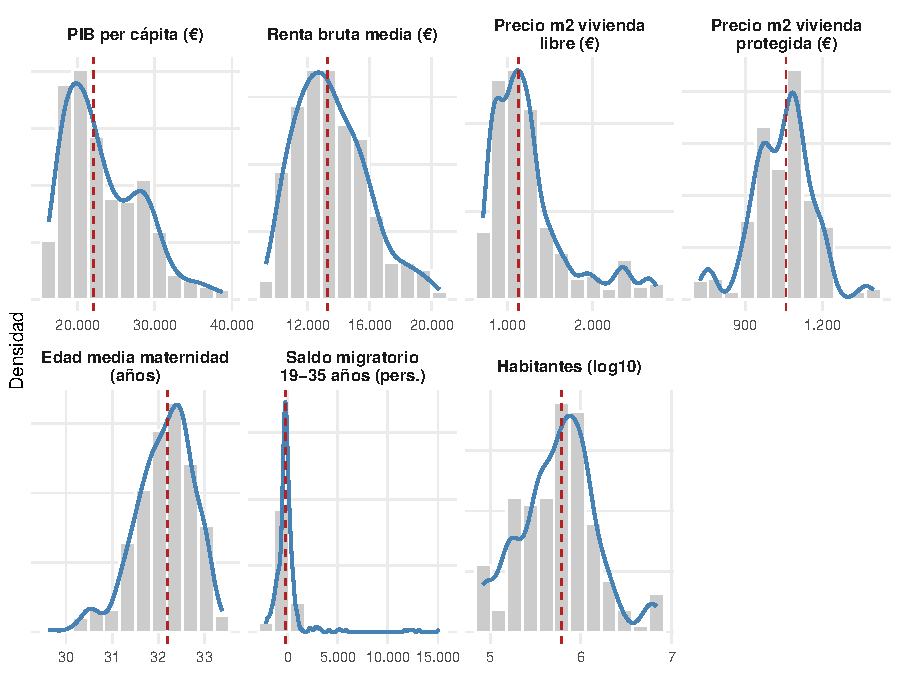
\includegraphics[width=1\linewidth]{plantilla_proyecto_aed_files/figure-latex/fig-univ-1-1} 

}

\caption{Distribución de las variables económicas y demográficas del panel provincial (2015-2021): histograma, densidad (azul) y mediana (rojo discontinuo). El número de habitantes se muestra en escala logarítmica.}\label{fig:fig-univ-1}
\end{figure}

La primera figura confirma gráficamente lo observado en las tablas. El
PIB per cápita y la renta bruta media tienen distribuciones unimodales
con cola derecha moderada; en el PIB se intuye además un segundo grupo
de provincias en torno a los 28.000-30.000 €. El precio de la vivienda
libre es claramente asimétrico: la mayoría de las provincias se
concentra entre 800 y 1.400 €/m², mientras que un pequeño grupo formado
por Gipuzkoa, Madrid, Bizkaia, Barcelona, Illes Balears y Araba/Álava se
aproxima o supera los 2.000 €/m² en varios años y genera la cola
derecha. El precio de la vivienda protegida, en cambio, es casi
simétrico y se concentra en torno a 1.050 €/m². La edad media de
maternidad es unimodal con una cola izquierda corta, formada por
Almería, Ceuta, Melilla y Huelva, y el saldo migratorio joven se
concentra en un pico muy estrecho alrededor de cero con una cola derecha
muy larga, debida sobre todo a Madrid. El número de habitantes, en
escala logarítmica, presenta una masa principal entre 200.000 y un
millón de habitantes y una cola de provincias muy grandes (Madrid y
Barcelona).

\begin{figure}[H]

{\centering 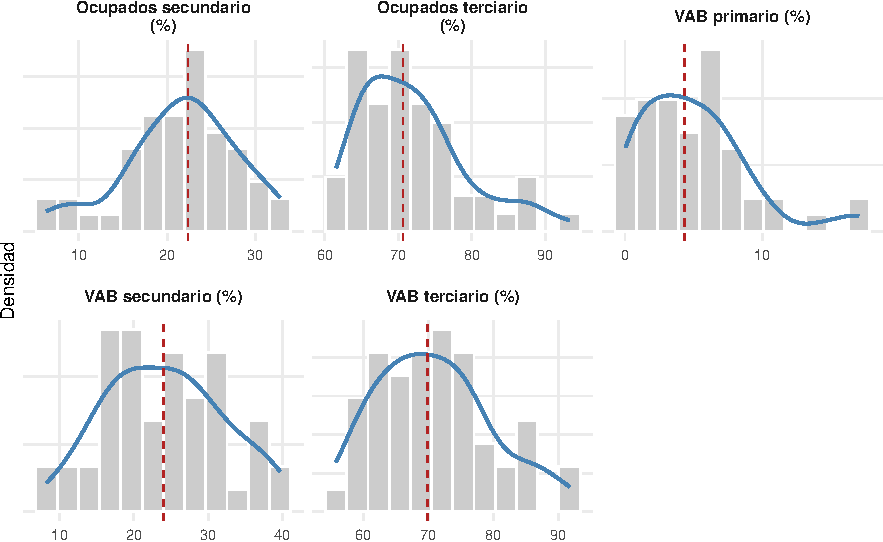
\includegraphics[width=1\linewidth]{plantilla_proyecto_aed_files/figure-latex/fig-univ-2-1} 

}

\caption{Distribución de la estructura productiva provincial: porcentaje de ocupados (fila superior) y de VAB (fila inferior) por sector.}\label{fig:fig-univ-2}
\end{figure}

La estructura productiva (segunda figura) refleja una economía
claramente terciarizada, con diferencias notables entre sectores. El
peso del terciario es unimodal y se centra en torno al 70 \%, con una
cola derecha de provincias muy terciarizadas (Melilla, Ceuta, Las
Palmas, Santa Cruz de Tenerife y Madrid superan en promedio el 85 \%),
que en el VAB aparece como un segundo bulto cercano al 85 \%. El
secundario es casi simétrico y alcanza sus mayores valores en provincias
industriales del interior y del norte (Burgos, Castellón, Araba/Álava,
Navarra, Guadalajara y Palencia superan el 35 \% del VAB). El primario
se concentra por debajo del 10 \%, con una cola larga debida a
provincias agrarias como Almería y Huelva, mientras que Madrid, Ceuta y
Melilla tienen un peso prácticamente nulo. Para cada sector, la
distribución de ocupados y de VAB es similar, pero el primario pesa más
en el empleo (7,0 \%) que en el VAB (5,4 \%), y el secundario menos
(21,2 \% frente a 24,1 \%), lo que sugiere una productividad relativa
menor del sector agrario.

\begin{figure}[H]

{\centering 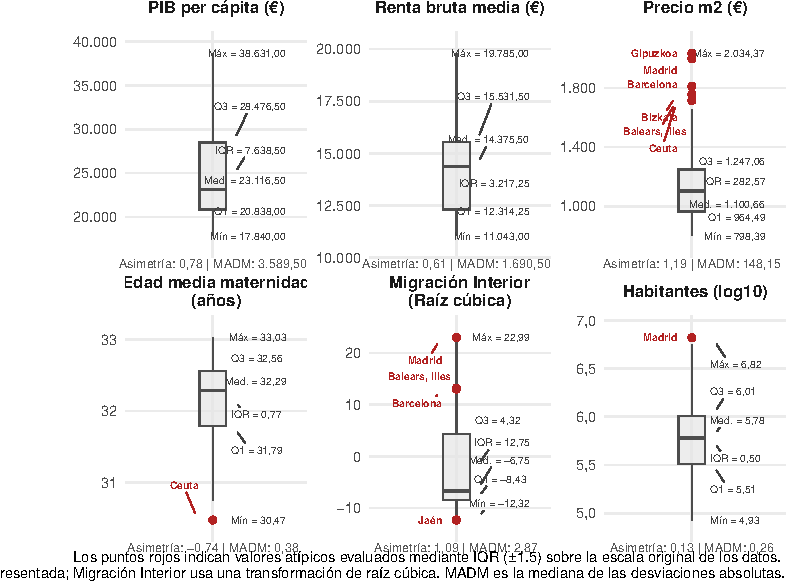
\includegraphics[width=1\linewidth]{plantilla_proyecto_aed_files/figure-latex/fig-univ-3-1} 

}

\caption{Distribución provincial por año de las variables clave. Los puntos rojos son valores fuera de 1,5 veces el rango intercuartílico.}\label{fig:fig-univ-3}
\end{figure}

La distribución anual (tercera figura) muestra que la forma de las
variables se mantiene estable. El PIB per cápita tiene una mediana que
crece de forma moderada hasta 2019, cae en 2020 y se recupera en 2021,
mientras que la renta bruta media sube de forma sostenida y sin caída en
2020. El precio de la vivienda libre mantiene una mediana casi
constante, y las provincias de precio elevado aparecen como valores
extremos en todos los años. La edad media de maternidad aumenta
gradualmente, con los valores bajos de Ceuta y Melilla como extremos. El
saldo migratorio joven se mantiene centrado en torno a cero con extremos
positivos en todos los años, y en 2020 y 2021 la caja se estrecha de
forma visible, es decir, hay menos movilidad entre provincias. El peso
del VAB terciario apenas varía. Los puntos rojos señalan valores fuera
del rango de Tukey con fines descriptivos; su tratamiento se discute en
la sección de valores atípicos.

\begin{table}[H]
\centering
\small
\resizebox{\ifdim\width>\linewidth\linewidth\else\width\fi}{!}{%

\begin{tabular}{lrr}
\toprule
Variable & W & p-valor\\
\midrule
PIB per cápita (€) & 0,932 & <0,001\\
Renta bruta media (€) & 0,969 & <0,001\\
Precio m² vivienda libre (€) & 0,838 & <0,001\\
Precio m² vivienda protegida (€) & 0,975 & <0,001\\
Edad media maternidad (años) & 0,971 & <0,001\\
Saldo migratorio 19-35 años (pers.) & 0,465 & <0,001\\
Habitantes & 0,568 & <0,001\\
Ocupados primario (\%) & 0,883 & <0,001\\
Ocupados secundario (\%) & 0,986 & 0,002\\
Ocupados terciario (\%) & 0,952 & <0,001\\
VAB primario (\%) & 0,912 & <0,001\\
VAB secundario (\%) & 0,988 & 0,005\\
VAB terciario (\%) & 0,961 & <0,001\\
Habitantes (log10) & 0,977 & <0,001\\
\bottomrule
\end{tabular}
}
\caption{Contraste de normalidad de Shapiro-Wilk (panel completo, orientativo por la repetición de provincias).}
\end{table}

El contraste rechaza la normalidad (p \textless{} 0,05) en las 14
variables evaluadas. Como con 364 observaciones el test detecta incluso
desviaciones pequeñas, es más informativo el valor del estadístico
\(W\): las variables más alejadas de la normalidad son el saldo
migratorio (\(W=0{,}47\)), el número de habitantes (\(W=0{,}57\)) y el
precio de la vivienda libre (\(W=0{,}84\)), mientras que los porcentajes
del secundario (ocupados y VAB) son los más próximos
(\(W \geq 0{,}98\)). Además, al repetirse cada provincia siete veces,
los \(p\)-valores deben tomarse como orientativos.

```\{r

\begin{figure}[H]

{\centering 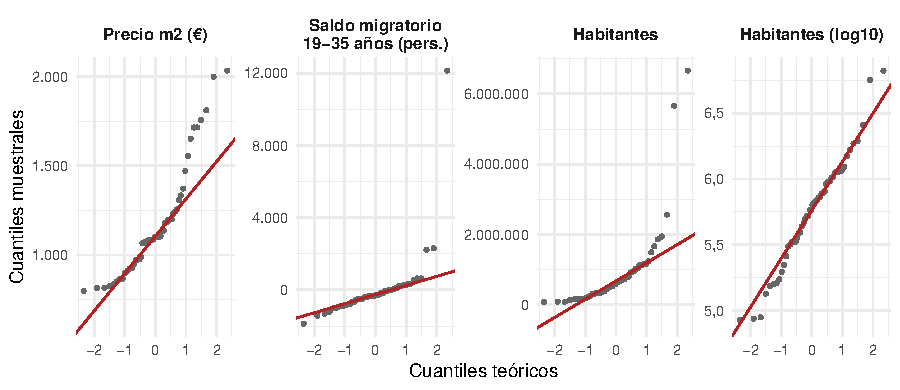
\includegraphics[width=1\linewidth]{plantilla_proyecto_aed_files/figure-latex/univariante-QQ-plot-1} 

}

\caption{Gráficos cuantil-cuantil de las variables más asimétricas; la línea roja es la normal teórica.}\label{fig:univariante-QQ-plot}
\end{figure}

Los gráficos cuantil-cuantil muestran dónde se produce la desviación. En
el precio de la vivienda libre y en el saldo migratorio los puntos se
separan de la recta por la cola derecha, que es mucho más pesada que la
normal; en el saldo migratorio hay además cuatro provincias-año con
saldos superiores a 10.000 personas, todas muy alejadas del resto. En el
número de habitantes, Madrid y Barcelona forman un grupo aparte en la
cola superior. La transformación logarítmica corrige casi por completo
esta desviación: los puntos de \(\log_{10}\)(habitantes) siguen la
recta, salvo en los extremos inferior (Ceuta y Melilla) y superior
(Madrid y Barcelona), y \(W\) pasa de 0,57 a 0,98. Estas desviaciones,
junto con los valores atípicos estructurales, apoyan el uso de la
correlación de Spearman en el análisis bivariante y de la escala
logarítmica para las variables de tamaño.

\subsection{5.2 Análisis Bivariante y
Multivariante}\label{anuxe1lisis-bivariante-y-multivariante}

En esta sección cruzamos las variables para dar respuesta a las
preguntas planteadas en la introducción. Para ello, fijamos el análisis
en el año 2018.

Aproximamos el salario medio mediante la renta bruta media y englobamos
los datos de hostelería y turismo en el sector terciario. Calculamos el
esfuerzo inmobiliario, el peso de cada sector, la densidad poblacional y
normalizamos la migración joven (20-35 años) por cada 1.000 habitantes.

\begin{Shaded}
\begin{Highlighting}[]
\NormalTok{Anyo }\OtherTok{\textless{}{-}} \DecValTok{2018}

\CommentTok{\# Superficie provincial a partir de mapSpain (para la densidad)}
\NormalTok{areas\_prov }\OtherTok{\textless{}{-}} \FunctionTok{esp\_get\_prov}\NormalTok{() }\SpecialCharTok{\%\textgreater{}\%}
  \FunctionTok{mutate}\NormalTok{(}\AttributeTok{area\_km2 =} \FunctionTok{as.numeric}\NormalTok{(}\FunctionTok{st\_area}\NormalTok{(geometry)) }\SpecialCharTok{/} \FloatTok{1e6}\NormalTok{) }\SpecialCharTok{\%\textgreater{}\%}
  \FunctionTok{st\_drop\_geometry}\NormalTok{() }\SpecialCharTok{\%\textgreater{}\%}
  \FunctionTok{select}\NormalTok{(}\AttributeTok{id\_prov =}\NormalTok{ cpro, area\_km2)}

\NormalTok{df\_completo }\OtherTok{\textless{}{-}}\NormalTok{ df\_completo }\SpecialCharTok{\%\textgreater{}\%}
  \FunctionTok{left\_join}\NormalTok{(ine\_provincias, }\AttributeTok{by =} \FunctionTok{c}\NormalTok{(}\StringTok{"Provincia"} \OtherTok{=} \StringTok{"Provincia\_clean"}\NormalTok{)) }\SpecialCharTok{\%\textgreater{}\%} 
  \FunctionTok{left\_join}\NormalTok{(areas\_prov, }\AttributeTok{by =} \StringTok{"id\_prov"}\NormalTok{) }\SpecialCharTok{\%\textgreater{}\%}
  \FunctionTok{mutate}\NormalTok{(}
    \AttributeTok{peso\_primario     =}\NormalTok{ VAB\_Primario   }\SpecialCharTok{/}\NormalTok{ (VAB\_Primario}\SpecialCharTok{+}\NormalTok{VAB\_Secundario}\SpecialCharTok{+}\NormalTok{VAB\_Terciario),}
    \AttributeTok{peso\_secundario   =}\NormalTok{ VAB\_Secundario }\SpecialCharTok{/}\NormalTok{ (VAB\_Primario}\SpecialCharTok{+}\NormalTok{VAB\_Secundario}\SpecialCharTok{+}\NormalTok{VAB\_Terciario),}
    \AttributeTok{peso\_terciario    =}\NormalTok{ VAB\_Terciario  }\SpecialCharTok{/}\NormalTok{ (VAB\_Primario}\SpecialCharTok{+}\NormalTok{VAB\_Secundario}\SpecialCharTok{+}\NormalTok{VAB\_Terciario),}
    \AttributeTok{emp\_terciario     =}\NormalTok{ Personas\_Ocupadas\_Terciario }\SpecialCharTok{/}\NormalTok{ Personas\_Ocupadas\_Total,}
    \CommentTok{\# Años de renta bruta media necesarios para una vivienda de 80 m2}
    \AttributeTok{esfuerzo\_vivienda =}\NormalTok{ (Precio\_m2\_libre }\SpecialCharTok{*} \DecValTok{80}\NormalTok{) }\SpecialCharTok{/}\NormalTok{ RentaBrutaMedia,}
    \AttributeTok{mig\_joven\_1000    =}\NormalTok{ (Migracion\_Interior }\SpecialCharTok{/}\NormalTok{ Habitantes) }\SpecialCharTok{*} \DecValTok{1000}\NormalTok{,}
    \AttributeTok{log\_densidad      =} \FunctionTok{log10}\NormalTok{(Habitantes }\SpecialCharTok{/}\NormalTok{ area\_km2)}
\NormalTok{  ) }\SpecialCharTok{\%\textgreater{}\%}
  \FunctionTok{group\_by}\NormalTok{(Periodo) }\SpecialCharTok{\%\textgreater{}\%}
  \FunctionTok{mutate}\NormalTok{(}
    \CommentTok{\# Brecha: si es \textgreater{}1, la provincia genera más PIB que renta percibe vs la media nacional}
    \AttributeTok{brecha\_pib\_renta =}\NormalTok{ (PIB\_per\_capita }\SpecialCharTok{/} \FunctionTok{mean}\NormalTok{(PIB\_per\_capita, }\AttributeTok{na.rm =} \ConstantTok{TRUE}\NormalTok{)) }\SpecialCharTok{/}
\NormalTok{                       (RentaBrutaMedia }\SpecialCharTok{/} \FunctionTok{mean}\NormalTok{(RentaBrutaMedia, }\AttributeTok{na.rm =} \ConstantTok{TRUE}\NormalTok{))}
\NormalTok{  ) }\SpecialCharTok{\%\textgreater{}\%}
  \FunctionTok{ungroup}\NormalTok{() }\SpecialCharTok{\%\textgreater{}\%}
  \FunctionTok{mutate}\NormalTok{(}
    \AttributeTok{nivel\_terciarizacion =} \FunctionTok{case\_when}\NormalTok{(}
\NormalTok{      peso\_terciario }\SpecialCharTok{\textless{}} \FloatTok{0.65} \SpecialCharTok{\textasciitilde{}} \StringTok{"Baja (\textless{}65\%)"}\NormalTok{,}
\NormalTok{      peso\_terciario }\SpecialCharTok{\textgreater{}=} \FloatTok{0.65} \SpecialCharTok{\&}\NormalTok{ peso\_terciario }\SpecialCharTok{\textless{}=} \FloatTok{0.75} \SpecialCharTok{\textasciitilde{}} \StringTok{"Media (65{-}75\%)"}\NormalTok{,}
\NormalTok{      peso\_terciario }\SpecialCharTok{\textgreater{}} \FloatTok{0.75} \SpecialCharTok{\textasciitilde{}} \StringTok{"Alta (\textgreater{}75\%)"}
\NormalTok{    ),}
    \AttributeTok{nivel\_terciarizacion =} \FunctionTok{factor}\NormalTok{(nivel\_terciarizacion, }
                                  \AttributeTok{levels =} \FunctionTok{c}\NormalTok{(}\StringTok{"Baja (\textless{}65\%)"}\NormalTok{, }\StringTok{"Media (65{-}75\%)"}\NormalTok{, }\StringTok{"Alta (\textgreater{}75\%)"}\NormalTok{))}
\NormalTok{  )}

\NormalTok{df\_anio }\OtherTok{\textless{}{-}}\NormalTok{ df\_completo }\SpecialCharTok{\%\textgreater{}\%} 
  \FunctionTok{filter}\NormalTok{(Periodo }\SpecialCharTok{==}\NormalTok{ Anyo) }\SpecialCharTok{\%\textgreater{}\%}
  \FunctionTok{mutate}\NormalTok{(}
    \CommentTok{\# Filtramos el top 5 por arriba y por abajo para la Brecha PIB/Renta}
    \AttributeTok{label\_pib =} \FunctionTok{ifelse}\NormalTok{(}
      \FunctionTok{rank}\NormalTok{(brecha\_pib\_renta, }\AttributeTok{ties.method =} \StringTok{"first"}\NormalTok{) }\SpecialCharTok{\textless{}=} \DecValTok{5} \SpecialCharTok{|} \FunctionTok{rank}\NormalTok{(}\FunctionTok{desc}\NormalTok{(brecha\_pib\_renta), }\AttributeTok{ties.method =} \StringTok{"first"}\NormalTok{) }\SpecialCharTok{\textless{}=} \DecValTok{5}\NormalTok{,}
      \FunctionTok{as.character}\NormalTok{(Provincia), }
      \ConstantTok{NA}
\NormalTok{    ),}
    \CommentTok{\# Filtramos el top 5 por arriba y por abajo para el Esfuerzo Inmobiliario}
    \AttributeTok{label\_trampa =} \FunctionTok{ifelse}\NormalTok{(}
      \FunctionTok{rank}\NormalTok{(esfuerzo\_vivienda, }\AttributeTok{ties.method =} \StringTok{"first"}\NormalTok{) }\SpecialCharTok{\textless{}=} \DecValTok{5} \SpecialCharTok{|} \FunctionTok{rank}\NormalTok{(}\FunctionTok{desc}\NormalTok{(esfuerzo\_vivienda), }\AttributeTok{ties.method =} \StringTok{"first"}\NormalTok{) }\SpecialCharTok{\textless{}=} \DecValTok{5}\NormalTok{,}
      \FunctionTok{as.character}\NormalTok{(Provincia), }
      \ConstantTok{NA}
\NormalTok{    )}
\NormalTok{  )}
\end{Highlighting}
\end{Shaded}

\subsubsection{El espejismo del PIB}\label{el-espejismo-del-pib}

Analizamos la relación entre la riqueza generada (PIB per cápita) y la
percibida (Renta Bruta Media), así como la influencia del sector
terciario en la brecha entre ambas.

\begin{Shaded}
\begin{Highlighting}[]
\FunctionTok{ggplot}\NormalTok{(df\_anio, }\FunctionTok{aes}\NormalTok{(}\AttributeTok{x =}\NormalTok{ PIB\_per\_capita, }\AttributeTok{y =}\NormalTok{ RentaBrutaMedia)) }\SpecialCharTok{+} 
  \FunctionTok{geom\_point}\NormalTok{(}\FunctionTok{aes}\NormalTok{(}\AttributeTok{colour =}\NormalTok{ peso\_terciario), }\AttributeTok{size =} \DecValTok{3}\NormalTok{, }\AttributeTok{alpha =} \FloatTok{0.8}\NormalTok{) }\SpecialCharTok{+} 
  \FunctionTok{geom\_smooth}\NormalTok{(}\AttributeTok{method =} \StringTok{"lm"}\NormalTok{, }\AttributeTok{col =} \StringTok{"black"}\NormalTok{, }\AttributeTok{linetype =} \StringTok{"dashed"}\NormalTok{) }\SpecialCharTok{+} 
  \FunctionTok{geom\_text\_repel}\NormalTok{(}\FunctionTok{aes}\NormalTok{(}\AttributeTok{label =}\NormalTok{ label\_pib), }\AttributeTok{size =} \DecValTok{3}\NormalTok{, }\AttributeTok{max.overlaps =} \ConstantTok{Inf}\NormalTok{, }\AttributeTok{na.rm =} \ConstantTok{TRUE}\NormalTok{, }\AttributeTok{box.padding =} \FloatTok{0.5}\NormalTok{) }\SpecialCharTok{+} 
  \FunctionTok{labs}\NormalTok{(}
    \AttributeTok{title =} \StringTok{"Relación entre PIB per cápita y Renta Bruta Media"}\NormalTok{,}
    \AttributeTok{x =} \StringTok{"PIB per cápita (€)"}\NormalTok{,}
    \AttributeTok{y =} \StringTok{"Renta bruta media anual (€)"}\NormalTok{,}
    \AttributeTok{color =} \StringTok{"Peso del}\SpecialCharTok{\textbackslash{}n}\StringTok{Sector Terciario"}
\NormalTok{  ) }\SpecialCharTok{+} 
  \FunctionTok{theme\_minimal}\NormalTok{()}
\end{Highlighting}
\end{Shaded}

\begin{center}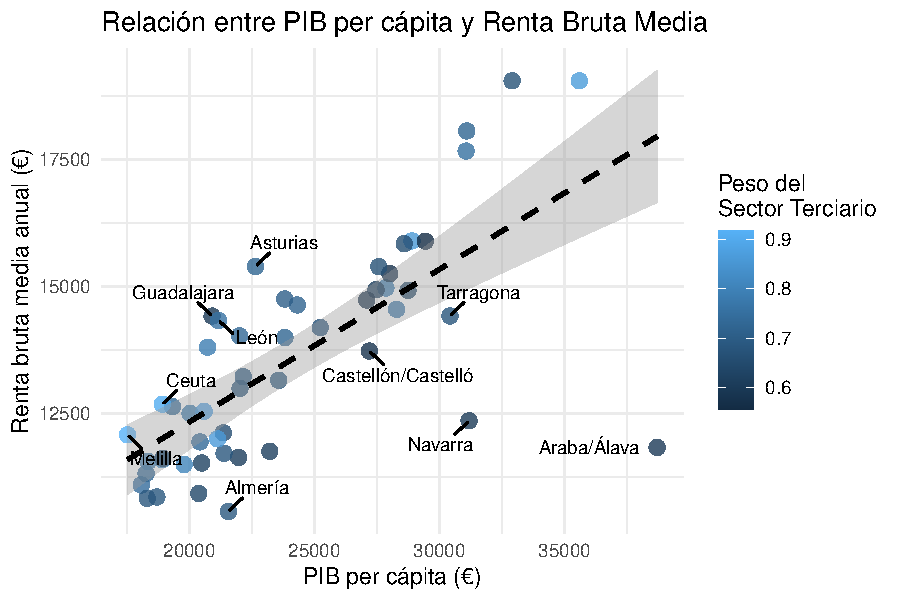
\includegraphics[width=1\linewidth]{plantilla_proyecto_aed_files/figure-latex/unnamed-chunk-20-1} \end{center}

\begin{Shaded}
\begin{Highlighting}[]
\CommentTok{\# Contraste de correlación: Brecha PIB/Renta vs Peso del sector terciario}
\FunctionTok{cor.test}\NormalTok{(df\_anio}\SpecialCharTok{$}\NormalTok{brecha\_pib\_renta, df\_anio}\SpecialCharTok{$}\NormalTok{peso\_terciario)}
\end{Highlighting}
\end{Shaded}

\begin{verbatim}
## 
##  Pearson's product-moment correlation
## 
## data:  df_anio$brecha_pib_renta and df_anio$peso_terciario
## t = -3.1375, df = 50, p-value = 0.002855
## alternative hypothesis: true correlation is not equal to 0
## 95 percent confidence interval:
##  -0.6108643 -0.1491874
## sample estimates:
##        cor 
## -0.4055754
\end{verbatim}

\begin{Shaded}
\begin{Highlighting}[]
\NormalTok{df\_anio }\SpecialCharTok{\%\textgreater{}\%} \FunctionTok{ggplot}\NormalTok{(}\FunctionTok{aes}\NormalTok{(}\AttributeTok{x =}\NormalTok{ brecha\_pib\_renta, }\AttributeTok{y =}\NormalTok{ peso\_terciario)) }\SpecialCharTok{+} 
  \FunctionTok{geom\_point}\NormalTok{(}\AttributeTok{colour =} \StringTok{"steelblue"}\NormalTok{) }\SpecialCharTok{+} 
  \FunctionTok{geom\_smooth}\NormalTok{(}\AttributeTok{method =} \StringTok{"lm"}\NormalTok{, }\AttributeTok{col =} \StringTok{"black"}\NormalTok{, }\AttributeTok{linetype =} \StringTok{"dashed"}\NormalTok{) }\SpecialCharTok{+}
  \FunctionTok{geom\_text\_repel}\NormalTok{(}\FunctionTok{aes}\NormalTok{(}\AttributeTok{label =}\NormalTok{ label\_pib), }\AttributeTok{size =} \DecValTok{3}\NormalTok{, }\AttributeTok{max.overlaps =} \ConstantTok{Inf}\NormalTok{, }\AttributeTok{na.rm =} \ConstantTok{TRUE}\NormalTok{, }\AttributeTok{box.padding =} \FloatTok{0.5}\NormalTok{) }\SpecialCharTok{+}
  \FunctionTok{labs}\NormalTok{(}
    \AttributeTok{title =} \StringTok{"Relación entre la brecha PIB/Renta y el peso del sector terciario"}\NormalTok{,}
    \AttributeTok{x =} \StringTok{"Brecha PIB/Renta"}\NormalTok{,}
    \AttributeTok{y =} \StringTok{"Peso del sector terciario"}\NormalTok{,}
    \AttributeTok{color =} \StringTok{"Peso del}\SpecialCharTok{\textbackslash{}n}\StringTok{Sector Terciario"}
\NormalTok{  ) }\SpecialCharTok{+} 
  \FunctionTok{theme\_minimal}\NormalTok{()}
\end{Highlighting}
\end{Shaded}

\begin{center}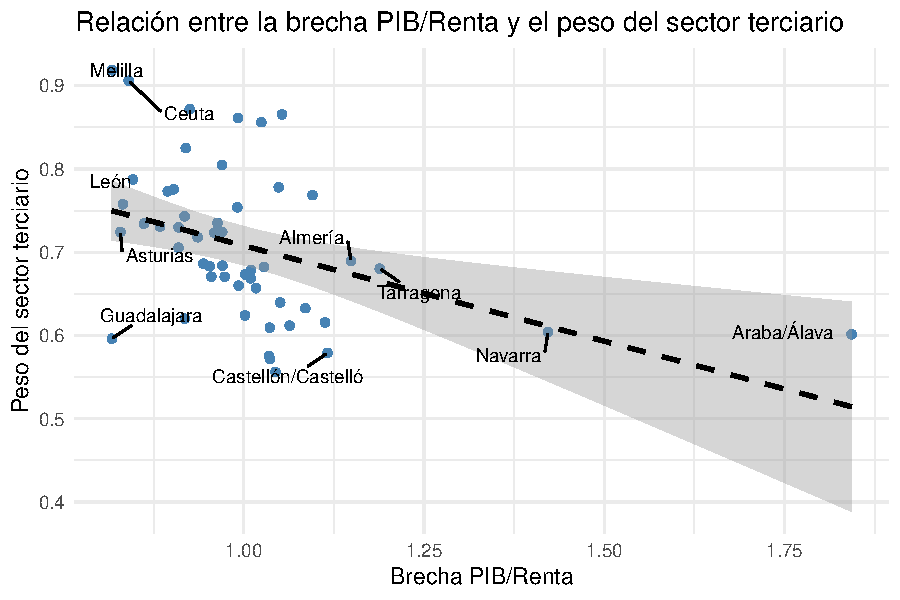
\includegraphics[width=1\linewidth]{plantilla_proyecto_aed_files/figure-latex/unnamed-chunk-20-2} \end{center}

Interpretación: Observamos si las provincias que quedan por debajo de la
línea de tendencia (mayor brecha, perciben menos renta de la que
producen) coinciden con altos porcentajes del sector terciario. El
contraste de hipótesis evalúa la significancia estadística de esta
correlación.

Para visualizar geográficamente dónde se concentra esta brecha (dónde se
produce más de lo que repercute en el salario de los trabajadores),
representamos los datos en un mapa a nivel provincial.

\begin{Shaded}
\begin{Highlighting}[]
\CommentTok{\# Unimos los datos espaciales con nuestro dataframe}
\NormalTok{mapa\_sf }\OtherTok{\textless{}{-}} \FunctionTok{esp\_get\_prov}\NormalTok{() }\SpecialCharTok{\%\textgreater{}\%}
  \FunctionTok{inner\_join}\NormalTok{(df\_anio, }\AttributeTok{by =} \FunctionTok{c}\NormalTok{(}\StringTok{"cpro"} \OtherTok{=} \StringTok{"id\_prov"}\NormalTok{))}

\FunctionTok{ggplot}\NormalTok{(mapa\_sf) }\SpecialCharTok{+}
  \FunctionTok{geom\_sf}\NormalTok{(}\FunctionTok{aes}\NormalTok{(}\AttributeTok{fill =}\NormalTok{ brecha\_pib\_renta), }\AttributeTok{color =} \StringTok{"white"}\NormalTok{, }\AttributeTok{size =} \FloatTok{0.1}\NormalTok{) }\SpecialCharTok{+}
  \FunctionTok{scale\_fill\_gradient2}\NormalTok{(}
    \AttributeTok{low =} \StringTok{"steelblue"}\NormalTok{, }\AttributeTok{mid =} \StringTok{"white"}\NormalTok{, }\AttributeTok{high =} \StringTok{"darkred"}\NormalTok{, }
    \AttributeTok{midpoint =} \DecValTok{1}\NormalTok{, }\AttributeTok{name =} \StringTok{"Brecha}\SpecialCharTok{\textbackslash{}n}\StringTok{(\textgreater{}1 peor)"}
\NormalTok{  ) }\SpecialCharTok{+}
  \FunctionTok{labs}\NormalTok{(}
    \AttributeTok{title =} \StringTok{"Mapa de la Brecha entre PIB y Renta Bruta"}\NormalTok{,}
    \AttributeTok{subtitle =} \StringTok{"Zonas en rojo indican mayor desconexión entre la riqueza generada y la renta percibida"}
\NormalTok{  ) }\SpecialCharTok{+}
  \FunctionTok{theme\_void}\NormalTok{()}
\end{Highlighting}
\end{Shaded}

\begin{center}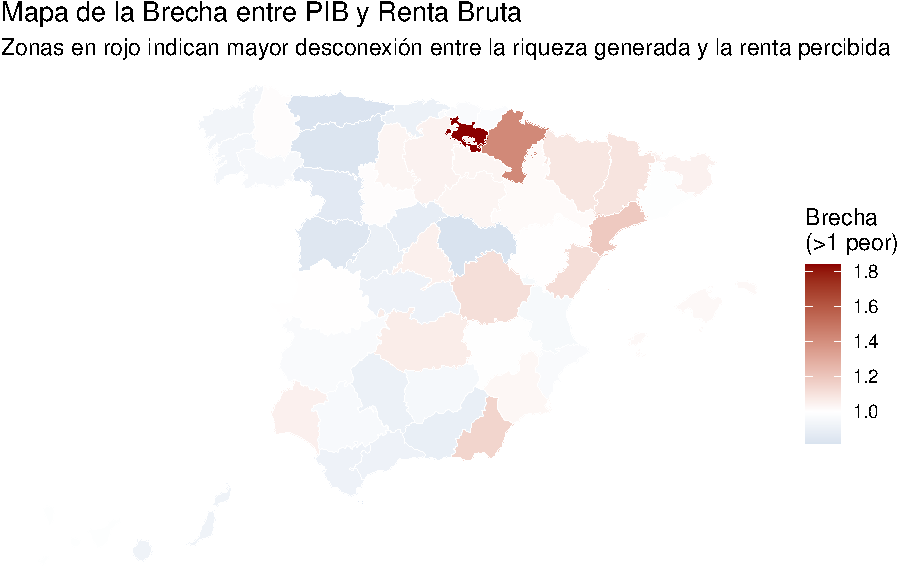
\includegraphics[width=1\linewidth]{plantilla_proyecto_aed_files/figure-latex/unnamed-chunk-21-1} \end{center}

\subsubsection{La trampa del sector
servicios}\label{la-trampa-del-sector-servicios}

Evaluamos cómo la dependencia del sector terciario presiona el coste de
la vivienda y cómo afecta a la expulsión de población joven.

\begin{Shaded}
\begin{Highlighting}[]
\FunctionTok{ggplot}\NormalTok{(df\_anio, }\FunctionTok{aes}\NormalTok{(}\AttributeTok{x =}\NormalTok{ emp\_terciario, }\AttributeTok{y =}\NormalTok{ esfuerzo\_vivienda)) }\SpecialCharTok{+}
  \FunctionTok{geom\_point}\NormalTok{(}\AttributeTok{alpha =} \FloatTok{0.7}\NormalTok{, }\AttributeTok{color =} \StringTok{"darkred"}\NormalTok{, }\AttributeTok{size =} \DecValTok{3}\NormalTok{) }\SpecialCharTok{+}
  \FunctionTok{geom\_smooth}\NormalTok{(}\AttributeTok{method =} \StringTok{"lm"}\NormalTok{, }\AttributeTok{se =} \ConstantTok{TRUE}\NormalTok{, }\AttributeTok{color =} \StringTok{"black"}\NormalTok{) }\SpecialCharTok{+}
  \FunctionTok{geom\_text\_repel}\NormalTok{(}\FunctionTok{aes}\NormalTok{(}\AttributeTok{label =}\NormalTok{ label\_trampa), }\AttributeTok{size =} \DecValTok{3}\NormalTok{, }\AttributeTok{max.overlaps =} \ConstantTok{Inf}\NormalTok{, }\AttributeTok{na.rm =} \ConstantTok{TRUE}\NormalTok{, }\AttributeTok{box.padding =} \FloatTok{0.5}\NormalTok{) }\SpecialCharTok{+}
  \FunctionTok{scale\_x\_continuous}\NormalTok{(}\AttributeTok{labels =}\NormalTok{ scales}\SpecialCharTok{::}\NormalTok{percent) }\SpecialCharTok{+}
  \FunctionTok{labs}\NormalTok{(}
    \AttributeTok{title =} \StringTok{"Empleo en el Sector Terciario vs Esfuerzo Inmobiliario"}\NormalTok{,}
    \AttributeTok{x =} \StringTok{"Proporción de empleo en el sector terciario"}\NormalTok{,}
    \AttributeTok{y =} \StringTok{"Años de renta para vivienda de 80m²"}
\NormalTok{  ) }\SpecialCharTok{+}
  \FunctionTok{theme\_minimal}\NormalTok{()}
\end{Highlighting}
\end{Shaded}

\begin{center}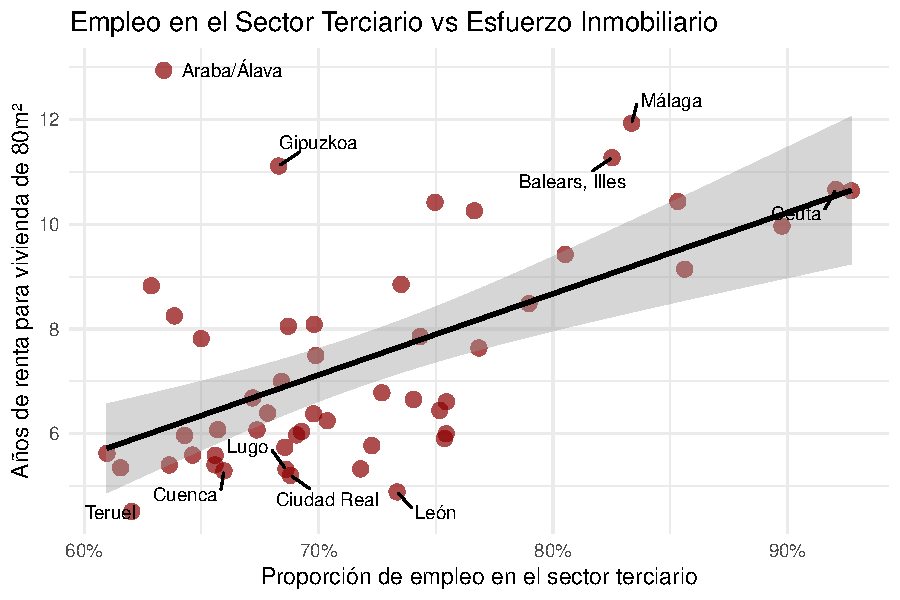
\includegraphics[width=1\linewidth]{plantilla_proyecto_aed_files/figure-latex/unnamed-chunk-22-1} \end{center}

\begin{Shaded}
\begin{Highlighting}[]
\CommentTok{\# Contraste: Empleo terciario y esfuerzo inmobiliario}
\FunctionTok{cor.test}\NormalTok{(df\_anio}\SpecialCharTok{$}\NormalTok{emp\_terciario, df\_anio}\SpecialCharTok{$}\NormalTok{esfuerzo\_vivienda)}
\end{Highlighting}
\end{Shaded}

\begin{verbatim}
## 
##  Pearson's product-moment correlation
## 
## data:  df_anio$emp_terciario and df_anio$esfuerzo_vivienda
## t = 4.9177, df = 50, p-value = 9.869e-06
## alternative hypothesis: true correlation is not equal to 0
## 95 percent confidence interval:
##  0.3530815 0.7301037
## sample estimates:
##       cor 
## 0.5709658
\end{verbatim}

\begin{Shaded}
\begin{Highlighting}[]
\CommentTok{\# Contraste: Empleo terciario y migración joven (expulsión)}
\FunctionTok{cor.test}\NormalTok{(df\_anio}\SpecialCharTok{$}\NormalTok{emp\_terciario, df\_anio}\SpecialCharTok{$}\NormalTok{mig\_joven\_1000)}
\end{Highlighting}
\end{Shaded}

\begin{verbatim}
## 
##  Pearson's product-moment correlation
## 
## data:  df_anio$emp_terciario and df_anio$mig_joven_1000
## t = 2.0101, df = 50, p-value = 0.04983
## alternative hypothesis: true correlation is not equal to 0
## 95 percent confidence interval:
##  0.0005761889 0.5083971859
## sample estimates:
##       cor 
## 0.2734335
\end{verbatim}

Para contrastar de forma más robusta si el modelo productivo discrimina
el acceso a la vivienda, agrupamos las provincias por su sector
económico predominante mediante un boxplot.

\begin{Shaded}
\begin{Highlighting}[]
\FunctionTok{ggplot}\NormalTok{(df\_anio, }\FunctionTok{aes}\NormalTok{(}\AttributeTok{x =}\NormalTok{ nivel\_terciarizacion, }\AttributeTok{y =}\NormalTok{ esfuerzo\_vivienda, }\AttributeTok{fill =}\NormalTok{ nivel\_terciarizacion)) }\SpecialCharTok{+}
  \FunctionTok{geom\_boxplot}\NormalTok{(}\AttributeTok{alpha =} \FloatTok{0.7}\NormalTok{, }\AttributeTok{outlier.color =} \StringTok{"red"}\NormalTok{, }\AttributeTok{outlier.size =} \DecValTok{2}\NormalTok{) }\SpecialCharTok{+}
  \FunctionTok{geom\_jitter}\NormalTok{(}\AttributeTok{width =} \FloatTok{0.15}\NormalTok{, }\AttributeTok{alpha =} \FloatTok{0.5}\NormalTok{, }\AttributeTok{color =} \StringTok{"darkslategrey"}\NormalTok{) }\SpecialCharTok{+}
  \FunctionTok{scale\_fill\_brewer}\NormalTok{(}\AttributeTok{palette =} \StringTok{"Oranges"}\NormalTok{) }\SpecialCharTok{+}
  \FunctionTok{labs}\NormalTok{(}
    \AttributeTok{title =} \StringTok{"Distribución del Esfuerzo Inmobiliario según Grado de Terciarización"}\NormalTok{,}
    \AttributeTok{x =} \StringTok{"Peso del Sector Terciario en el VAB"}\NormalTok{,}
    \AttributeTok{y =} \StringTok{"Años de renta para vivienda (80m²)"}\NormalTok{,}
    \AttributeTok{fill =} \StringTok{"Terciarización"}
\NormalTok{  ) }\SpecialCharTok{+}
  \FunctionTok{theme\_minimal}\NormalTok{() }\SpecialCharTok{+}
  \FunctionTok{theme}\NormalTok{(}\AttributeTok{legend.position =} \StringTok{"none"}\NormalTok{)}
\end{Highlighting}
\end{Shaded}

\begin{center}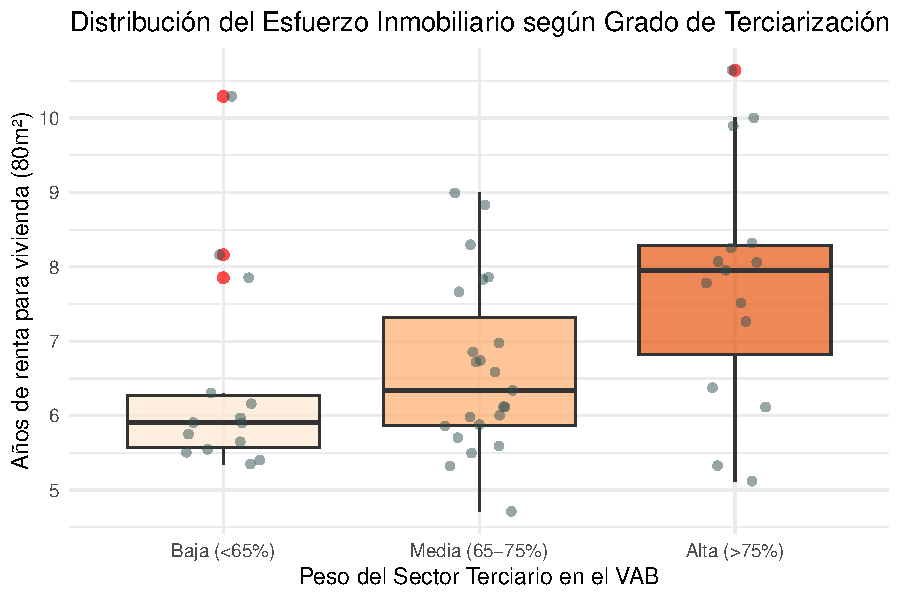
\includegraphics[width=1\linewidth]{plantilla_proyecto_aed_files/figure-latex/unnamed-chunk-23-1} \end{center}

Interpretación: Este diagrama de cajas nos permite evaluar si las
provincias fuertemente terciarizadas tienen una mediana de esfuerzo
inmobiliario significativamente superior frente a aquellas sostenidas
por el sector primario o secundario, así como detectar provincias
atípicas (outliers).

\subsubsection{El coste de la
maternidad}\label{el-coste-de-la-maternidad}

Buscamos evidenciar si el endurecimiento del mercado inmobiliario
(esfuerzo para acceder a una vivienda) retrasa la edad media a la
maternidad.

\begin{Shaded}
\begin{Highlighting}[]
\FunctionTok{ggplot}\NormalTok{(df\_anio, }\FunctionTok{aes}\NormalTok{(}\AttributeTok{x =}\NormalTok{ esfuerzo\_vivienda, }\AttributeTok{y =}\NormalTok{ Edad\_Media\_Maternidad)) }\SpecialCharTok{+}
  \FunctionTok{geom\_point}\NormalTok{(}\FunctionTok{aes}\NormalTok{(}\AttributeTok{size =}\NormalTok{ Habitantes), }\AttributeTok{alpha =} \FloatTok{0.6}\NormalTok{, }\AttributeTok{color =} \StringTok{"steelblue"}\NormalTok{) }\SpecialCharTok{+}
  \FunctionTok{geom\_smooth}\NormalTok{(}\AttributeTok{method =} \StringTok{"loess"}\NormalTok{, }\AttributeTok{color =} \StringTok{"darkorange"}\NormalTok{, }\AttributeTok{fill =} \StringTok{"lightgray"}\NormalTok{) }\SpecialCharTok{+}
  \FunctionTok{labs}\NormalTok{(}
    \AttributeTok{title =} \StringTok{"Esfuerzo Inmobiliario vs Edad de Maternidad"}\NormalTok{,}
    \AttributeTok{x =} \StringTok{"Años de renta necesarios para comprar una vivienda de 80m²"}\NormalTok{,}
    \AttributeTok{y =} \StringTok{"Edad Media a la Maternidad"}\NormalTok{,}
    \AttributeTok{size =} \StringTok{"Población"}
\NormalTok{  ) }\SpecialCharTok{+} \FunctionTok{scale\_size\_continuous}\NormalTok{(}\AttributeTok{labels =}\NormalTok{ scales}\SpecialCharTok{::}\NormalTok{comma) }\SpecialCharTok{+}
  \FunctionTok{theme\_minimal}\NormalTok{()}
\end{Highlighting}
\end{Shaded}

\begin{center}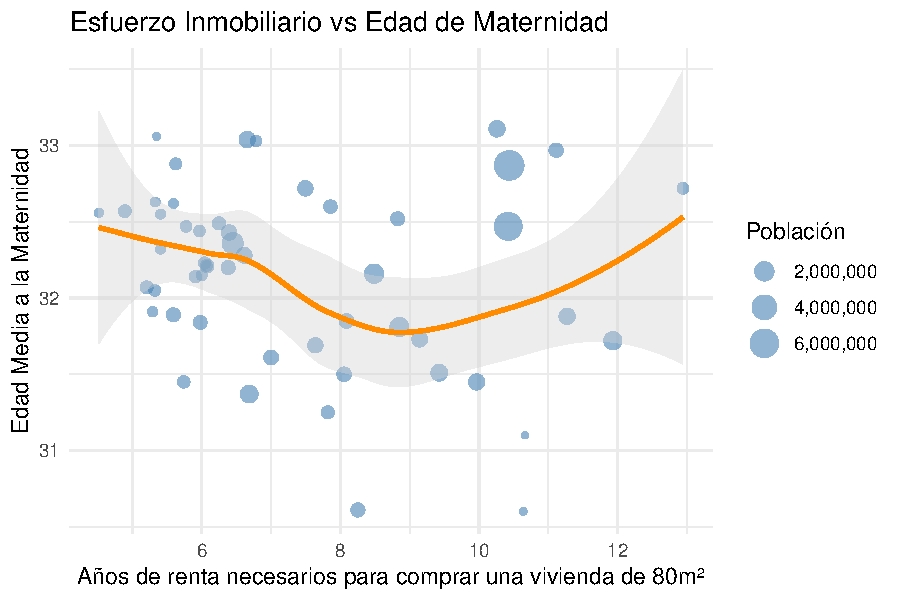
\includegraphics[width=1\linewidth]{plantilla_proyecto_aed_files/figure-latex/unnamed-chunk-24-1} \end{center}

\begin{Shaded}
\begin{Highlighting}[]
\CommentTok{\# Contraste de correlación lineal}
\FunctionTok{cor.test}\NormalTok{(df\_anio}\SpecialCharTok{$}\NormalTok{esfuerzo\_vivienda, df\_anio}\SpecialCharTok{$}\NormalTok{Edad\_Media\_Maternidad)}
\end{Highlighting}
\end{Shaded}

\begin{verbatim}
## 
##  Pearson's product-moment correlation
## 
## data:  df_anio$esfuerzo_vivienda and df_anio$Edad_Media_Maternidad
## t = -1.5027, df = 50, p-value = 0.1392
## alternative hypothesis: true correlation is not equal to 0
## 95 percent confidence interval:
##  -0.45495819  0.06894518
## sample estimates:
##        cor 
## -0.2078662
\end{verbatim}

Interpretación: La curva de ajuste local (LOESS) permite observar si
existe un crecimiento no lineal o un umbral crítico de esfuerzo
inmobiliario a partir del cual la edad de maternidad se dispara.

\subsubsection{El refugio industrial}\label{el-refugio-industrial}

Comprobamos si el tejido industrial funciona como fijador de población
joven y si se correlaciona con una densidad demográfica más equilibrada.

\begin{Shaded}
\begin{Highlighting}[]
\FunctionTok{ggplot}\NormalTok{(df\_anio, }\FunctionTok{aes}\NormalTok{(}\AttributeTok{x =}\NormalTok{ peso\_secundario, }\AttributeTok{y =}\NormalTok{ mig\_joven\_1000)) }\SpecialCharTok{+}
  \FunctionTok{geom\_point}\NormalTok{(}\AttributeTok{color =} \StringTok{"forestgreen"}\NormalTok{, }\AttributeTok{size =} \DecValTok{3}\NormalTok{, }\AttributeTok{alpha =} \FloatTok{0.7}\NormalTok{) }\SpecialCharTok{+}
  \FunctionTok{geom\_hline}\NormalTok{(}\AttributeTok{yintercept =} \DecValTok{0}\NormalTok{, }\AttributeTok{linetype =} \StringTok{"dashed"}\NormalTok{, }\AttributeTok{color =} \StringTok{"red"}\NormalTok{) }\SpecialCharTok{+}
  \FunctionTok{geom\_smooth}\NormalTok{(}\AttributeTok{method =} \StringTok{"lm"}\NormalTok{, }\AttributeTok{color =} \StringTok{"black"}\NormalTok{) }\SpecialCharTok{+}
  \FunctionTok{scale\_x\_continuous}\NormalTok{(}\AttributeTok{labels =}\NormalTok{ scales}\SpecialCharTok{::}\NormalTok{percent) }\SpecialCharTok{+}
  \FunctionTok{labs}\NormalTok{(}
    \AttributeTok{title =} \StringTok{"Peso del Sector Industrial vs Saldo Migratorio Joven"}\NormalTok{,}
    \AttributeTok{x =} \StringTok{"Peso del sector secundario en el VAB"}\NormalTok{,}
    \AttributeTok{y =} \StringTok{"Saldo migratorio interior (20{-}35 años) por mil hab."}
\NormalTok{  ) }\SpecialCharTok{+}
  \FunctionTok{theme\_minimal}\NormalTok{()}
\end{Highlighting}
\end{Shaded}

\begin{center}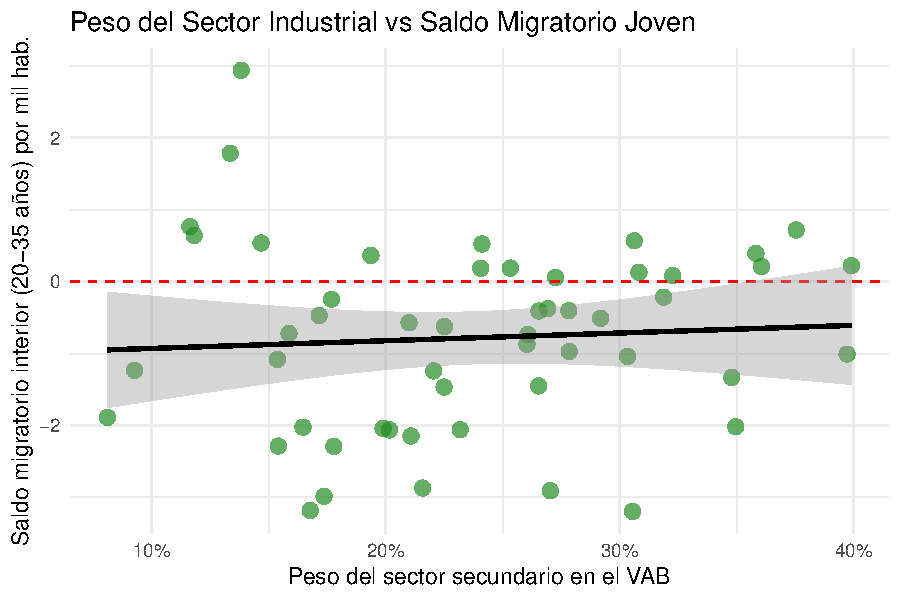
\includegraphics[width=1\linewidth]{plantilla_proyecto_aed_files/figure-latex/unnamed-chunk-25-1} \end{center}

\begin{Shaded}
\begin{Highlighting}[]
\CommentTok{\# Contraste: Industrialización vs retención de jóvenes}
\FunctionTok{cor.test}\NormalTok{(df\_anio}\SpecialCharTok{$}\NormalTok{peso\_secundario, df\_anio}\SpecialCharTok{$}\NormalTok{mig\_joven\_1000)}
\end{Highlighting}
\end{Shaded}

\begin{verbatim}
## 
##  Pearson's product-moment correlation
## 
## data:  df_anio$peso_secundario and df_anio$mig_joven_1000
## t = 0.47009, df = 50, p-value = 0.6403
## alternative hypothesis: true correlation is not equal to 0
## 95 percent confidence interval:
##  -0.2103748  0.3332023
## sample estimates:
##        cor 
## 0.06633382
\end{verbatim}

\begin{Shaded}
\begin{Highlighting}[]
\CommentTok{\# Contraste: Industrialización vs Densidad poblacional}
\FunctionTok{cor.test}\NormalTok{(df\_anio}\SpecialCharTok{$}\NormalTok{peso\_secundario, df\_anio}\SpecialCharTok{$}\NormalTok{log\_densidad)}
\end{Highlighting}
\end{Shaded}

\begin{verbatim}
## 
##  Pearson's product-moment correlation
## 
## data:  df_anio$peso_secundario and df_anio$log_densidad
## t = -3.0911, df = 50, p-value = 0.003256
## alternative hypothesis: true correlation is not equal to 0
## 95 percent confidence interval:
##  -0.6070864 -0.1433112
## sample estimates:
##        cor 
## -0.4005463
\end{verbatim}

Para observar con claridad cuáles son las provincias que lideran la
atracción y expulsión de jóvenes, generamos un barplot divergente
aislando el top 10 y bottom 10.

\begin{Shaded}
\begin{Highlighting}[]
\NormalTok{df\_anio }\SpecialCharTok{\%\textgreater{}\%}
  \FunctionTok{arrange}\NormalTok{(}\FunctionTok{desc}\NormalTok{(mig\_joven\_1000)) }\SpecialCharTok{\%\textgreater{}\%}
  \CommentTok{\# Seleccionamos las 10 con mayor saldo positivo y las 10 con mayor saldo negativo}
  \FunctionTok{filter}\NormalTok{(}\FunctionTok{row\_number}\NormalTok{() }\SpecialCharTok{\textless{}=} \DecValTok{10} \SpecialCharTok{|} \FunctionTok{row\_number}\NormalTok{() }\SpecialCharTok{\textgreater{}=}\NormalTok{ (}\FunctionTok{n}\NormalTok{() }\SpecialCharTok{{-}} \DecValTok{9}\NormalTok{)) }\SpecialCharTok{\%\textgreater{}\%}
  \FunctionTok{mutate}\NormalTok{(}\AttributeTok{Provincia =} \FunctionTok{fct\_reorder}\NormalTok{(Provincia, mig\_joven\_1000)) }\SpecialCharTok{\%\textgreater{}\%}
  \FunctionTok{ggplot}\NormalTok{(}\FunctionTok{aes}\NormalTok{(}\AttributeTok{x =}\NormalTok{ mig\_joven\_1000, }\AttributeTok{y =}\NormalTok{ Provincia, }\AttributeTok{fill =}\NormalTok{ mig\_joven\_1000 }\SpecialCharTok{\textgreater{}} \DecValTok{0}\NormalTok{)) }\SpecialCharTok{+}
  \FunctionTok{geom\_col}\NormalTok{() }\SpecialCharTok{+}
  \FunctionTok{scale\_fill\_manual}\NormalTok{(}\AttributeTok{values =} \FunctionTok{c}\NormalTok{(}\StringTok{"TRUE"} \OtherTok{=} \StringTok{"forestgreen"}\NormalTok{, }\StringTok{"FALSE"} \OtherTok{=} \StringTok{"firebrick"}\NormalTok{)) }\SpecialCharTok{+}
  \FunctionTok{labs}\NormalTok{(}
    \AttributeTok{title =} \StringTok{"Top 10 Atracción vs Top 10 Expulsión }\SpecialCharTok{\textbackslash{}n}\StringTok{de Jóvenes (20{-}35 años)"}\NormalTok{,}
    \AttributeTok{subtitle =} \StringTok{"Saldo migratorio interno normalizado por mil habitantes"}\NormalTok{,}
    \AttributeTok{x =} \StringTok{"Migración Neta (Jóvenes / 1000 hab.)"}\NormalTok{,}
    \AttributeTok{y =} \ConstantTok{NULL}
\NormalTok{  ) }\SpecialCharTok{+}
  \FunctionTok{theme\_minimal}\NormalTok{() }\SpecialCharTok{+}
  \FunctionTok{theme}\NormalTok{(}\AttributeTok{legend.position =} \StringTok{"none"}\NormalTok{)}
\end{Highlighting}
\end{Shaded}

\begin{center}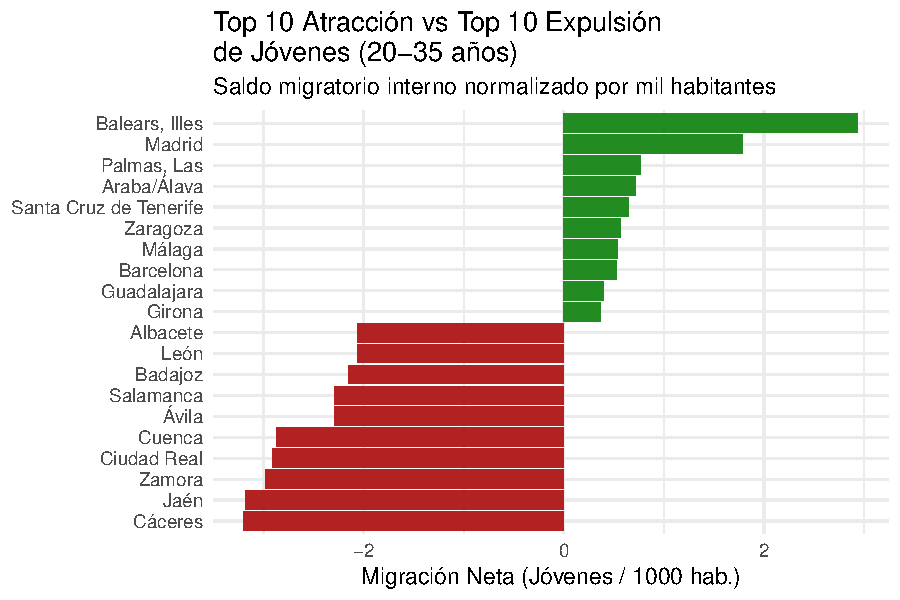
\includegraphics[width=1\linewidth]{plantilla_proyecto_aed_files/figure-latex/unnamed-chunk-26-1} \end{center}

\subsubsection{Visión multivariante
global}\label{visiuxf3n-multivariante-global}

Para resumir las dinámicas conjuntas, comenzamos con una matriz de
correlación.

\begin{Shaded}
\begin{Highlighting}[]
\CommentTok{\# Seleccionamos las variables continuas de interés}
\NormalTok{var\_corr }\OtherTok{\textless{}{-}}\NormalTok{ df\_anio }\SpecialCharTok{\%\textgreater{}\%}
  \FunctionTok{select}\NormalTok{(}
\NormalTok{    PIB\_per\_capita, RentaBrutaMedia, brecha\_pib\_renta, }
\NormalTok{    peso\_primario, peso\_secundario, peso\_terciario,}
\NormalTok{    esfuerzo\_vivienda, Edad\_Media\_Maternidad, mig\_joven\_1000, log\_densidad}
\NormalTok{  ) }\SpecialCharTok{\%\textgreater{}\%}
  \FunctionTok{drop\_na}\NormalTok{()}

\CommentTok{\# Calculamos matriz de correlación}
\NormalTok{matriz\_cor }\OtherTok{\textless{}{-}} \FunctionTok{cor}\NormalTok{(var\_corr)}

\CommentTok{\# Visualización}
\FunctionTok{corrplot}\NormalTok{(matriz\_cor, }
         \AttributeTok{method =} \StringTok{"color"}\NormalTok{, }
         \AttributeTok{type =} \StringTok{"upper"}\NormalTok{, }
         \AttributeTok{order =} \StringTok{"hclust"}\NormalTok{,}
         \AttributeTok{tl.col =} \StringTok{"black"}\NormalTok{, }
         \AttributeTok{tl.srt =} \DecValTok{45}\NormalTok{, }
         \AttributeTok{addCoef.col =} \StringTok{"black"}\NormalTok{, }
         \AttributeTok{number.cex =} \FloatTok{0.7}\NormalTok{,}
         \AttributeTok{diag =} \ConstantTok{FALSE}\NormalTok{)}
\end{Highlighting}
\end{Shaded}

\begin{center}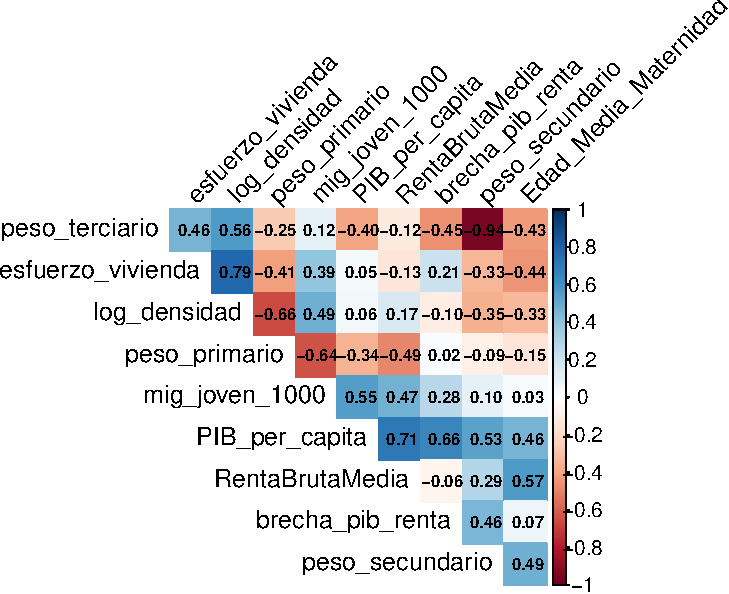
\includegraphics[width=1\linewidth]{plantilla_proyecto_aed_files/figure-latex/unnamed-chunk-27-1} \end{center}

Finalmente, para crear un perfil multidimensional sintético de las
tensiones sociodemográficas, generamos un heatmap estandarizado
(\texttt{geom\_tile}) de las 15 provincias más pobladas de España. Esto
nos muestra de un vistazo qué retos afronta cada polo demográfico.

\begin{Shaded}
\begin{Highlighting}[]
\CommentTok{\# Estandarizamos (Z{-}score) las variables para poder compararlas visualmente en la misma escala}
\NormalTok{df\_heat }\OtherTok{\textless{}{-}}\NormalTok{ df\_anio }\SpecialCharTok{\%\textgreater{}\%}
  \FunctionTok{slice\_max}\NormalTok{(Habitantes, }\AttributeTok{n =} \DecValTok{15}\NormalTok{) }\SpecialCharTok{\%\textgreater{}\%}
  \FunctionTok{select}\NormalTok{(Provincia, }
         \StringTok{\textasciigrave{}}\AttributeTok{PIB per cápita}\StringTok{\textasciigrave{}} \OtherTok{=}\NormalTok{ PIB\_per\_capita, }
         \StringTok{\textasciigrave{}}\AttributeTok{Renta Media}\StringTok{\textasciigrave{}} \OtherTok{=}\NormalTok{ RentaBrutaMedia, }
         \StringTok{\textasciigrave{}}\AttributeTok{Esfuerzo Inmobiliario}\StringTok{\textasciigrave{}} \OtherTok{=}\NormalTok{ esfuerzo\_vivienda, }
         \StringTok{\textasciigrave{}}\AttributeTok{Migración Joven}\StringTok{\textasciigrave{}} \OtherTok{=}\NormalTok{ mig\_joven\_1000, }
         \StringTok{\textasciigrave{}}\AttributeTok{Edad Maternidad}\StringTok{\textasciigrave{}} \OtherTok{=}\NormalTok{ Edad\_Media\_Maternidad) }\SpecialCharTok{\%\textgreater{}\%}
  \FunctionTok{pivot\_longer}\NormalTok{(}\AttributeTok{cols =} \SpecialCharTok{{-}}\NormalTok{Provincia, }\AttributeTok{names\_to =} \StringTok{"Variable"}\NormalTok{, }\AttributeTok{values\_to =} \StringTok{"Valor"}\NormalTok{) }\SpecialCharTok{\%\textgreater{}\%}
  \FunctionTok{group\_by}\NormalTok{(Variable) }\SpecialCharTok{\%\textgreater{}\%}
  \FunctionTok{mutate}\NormalTok{(}\AttributeTok{Valor\_Escalado =} \FunctionTok{scale}\NormalTok{(Valor)) }\SpecialCharTok{\%\textgreater{}\%}
  \FunctionTok{ungroup}\NormalTok{()}

\CommentTok{\# Extraemos el orden exacto ordenando por el esfuerzo inmobiliario}
\NormalTok{orden\_provincias }\OtherTok{\textless{}{-}}\NormalTok{ df\_heat }\SpecialCharTok{\%\textgreater{}\%}
  \FunctionTok{filter}\NormalTok{(Variable }\SpecialCharTok{==} \StringTok{"Esfuerzo Inmobiliario"}\NormalTok{) }\SpecialCharTok{\%\textgreater{}\%}
  \FunctionTok{arrange}\NormalTok{(Valor\_Escalado) }\SpecialCharTok{\%\textgreater{}\%}
  \FunctionTok{pull}\NormalTok{(Provincia)}

\CommentTok{\# Aplicamos el orden convirtiendo Provincia a un factor}
\NormalTok{df\_heat }\OtherTok{\textless{}{-}}\NormalTok{ df\_heat }\SpecialCharTok{\%\textgreater{}\%}
  \FunctionTok{mutate}\NormalTok{(}\AttributeTok{Provincia =} \FunctionTok{factor}\NormalTok{(Provincia, }\AttributeTok{levels =}\NormalTok{ orden\_provincias))}

\FunctionTok{ggplot}\NormalTok{(df\_heat, }\FunctionTok{aes}\NormalTok{(}\AttributeTok{x =}\NormalTok{ Variable, }\AttributeTok{y =}\NormalTok{ Provincia, }\AttributeTok{fill =}\NormalTok{ Valor\_Escalado)) }\SpecialCharTok{+}
  \FunctionTok{geom\_tile}\NormalTok{(}\AttributeTok{color =} \StringTok{"white"}\NormalTok{, }\AttributeTok{size =} \FloatTok{0.5}\NormalTok{) }\SpecialCharTok{+}
  \FunctionTok{scale\_fill\_gradient2}\NormalTok{(}\AttributeTok{low =} \StringTok{"royalblue"}\NormalTok{, }\AttributeTok{mid =} \StringTok{"white"}\NormalTok{, }\AttributeTok{high =} \StringTok{"darkred"}\NormalTok{, }\AttributeTok{midpoint =} \DecValTok{0}\NormalTok{) }\SpecialCharTok{+}
  \FunctionTok{labs}\NormalTok{(}
    \AttributeTok{title =} \StringTok{"Perfil Sociodemográfico de las 15 Provincias }\SpecialCharTok{\textbackslash{}n}\StringTok{Más Pobladas"}\NormalTok{,}
    \AttributeTok{subtitle =} \StringTok{"Valores estandarizados (Z{-}scores).}\SpecialCharTok{\textbackslash{}n}\StringTok{Provincias ordenadas por Esfuerzo Inmobiliario."}\NormalTok{,}
    \AttributeTok{x =} \ConstantTok{NULL}\NormalTok{,}
    \AttributeTok{y =} \ConstantTok{NULL}\NormalTok{,}
    \AttributeTok{fill =} \StringTok{"Desviación}\SpecialCharTok{\textbackslash{}n}\StringTok{Estándar"}
\NormalTok{  ) }\SpecialCharTok{+}
  \FunctionTok{theme\_minimal}\NormalTok{() }\SpecialCharTok{+}
  \FunctionTok{theme}\NormalTok{(}\AttributeTok{axis.text.x =} \FunctionTok{element\_text}\NormalTok{(}\AttributeTok{angle =} \DecValTok{45}\NormalTok{, }\AttributeTok{hjust =} \DecValTok{1}\NormalTok{))}
\end{Highlighting}
\end{Shaded}

\begin{center}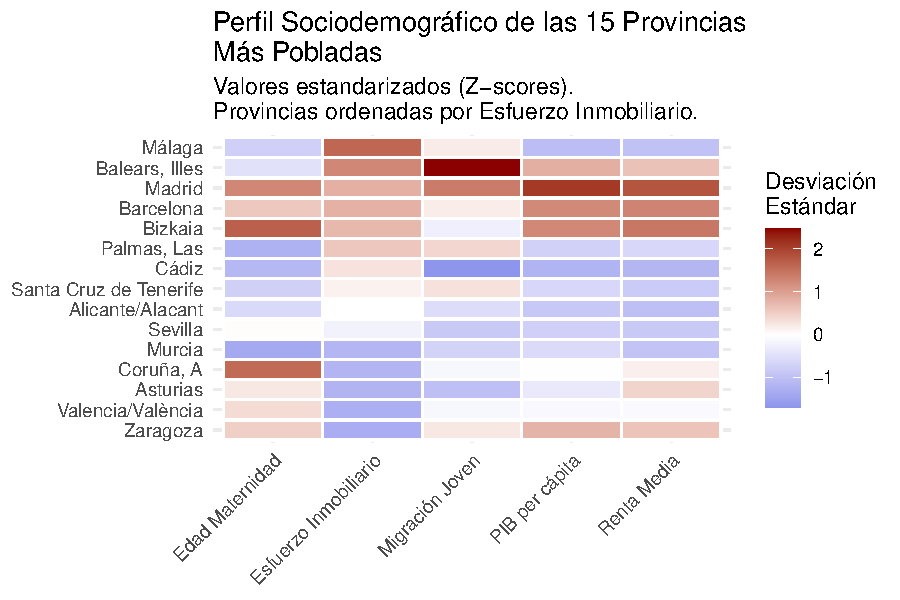
\includegraphics[width=1\linewidth]{plantilla_proyecto_aed_files/figure-latex/unnamed-chunk-28-1} \end{center}

\emph{Explicación detallada de los gráficos mostrados. ``Contar la
historia'' que revelan los datos. ¿Se confirman las hipótesis
iniciales?}

\section{6. Conclusiones Finales}\label{conclusiones-finales}

A partir del análisis exploratorio realizado, podemos extraer las
siguientes conclusiones:

\begin{itemize}
\tightlist
\item
  \textbf{Sobre el mercado inmobiliario y demografía:} (Respuesta a las
  preguntas 1 y 2).
\item
  \textbf{Sobre el modelo productivo y migración:} (Respuesta a las
  preguntas 3 y 4).
\item
  \textbf{Aportaciones adicionales:} (Limitaciones del estudio, posibles
  líneas futuras o reflexiones sobre los datos).
\end{itemize}

\newpage

\section{Referencias}\label{referencias}

\begin{itemize}
\tightlist
\item
  Instituto Nacional de Estadística (INE). (2026). \emph{Bases de datos
  provinciales}. Recuperado de
  \url{https://www.ine.es/dyngs/DAB/index.htm?cid=1722}
\item
  Xie, Y., Allaire, J. J., \& Grolemund, G. (2018). \emph{R Markdown:
  The Definitive Guide}. Chapman and Hall/CRC.
\end{itemize}

%%%%%%%%%%%%%%%%%%%%%%%%%%%%%%%%%%%%%%%%%%

\vspace{6pt}

%%%%%%%%%%%%%%%%%%%%%%%%%%%%%%%%%%%%%%%%%%
%% optional

% Only for the journal Methods and Protocols:
% If you wish to submit a video article, please do so with any other supplementary material.
% \supplementary{The following supporting information can be downloaded at: \linksupplementary{s1}, Figure S1: title; Table S1: title; Video S1: title. A supporting video article is available at doi: link.}

%%%%%%%%%%%%%%%%%%%%%%%%%%%%%%%%%%%%%%%%%%







%%%%%%%%%%%%%%%%%%%%%%%%%%%%%%%%%%%%%%%%%%
%% Optional

%% Only for journal Encyclopedia


%%%%%%%%%%%%%%%%%%%%%%%%%%%%%%%%%%%%%%%%%%
%% Optional
%%%%%%%%%%%%%%%%%%%%%%%%%%%%%%%%%%%%%%%%%%
\begin{adjustwidth}{-\extralength}{0cm}

%\printendnotes[custom] % Un-comment to print a list of endnotes



% If authors have biography, please use the format below
%\section*{Short Biography of Authors}
%\bio
%{\raisebox{-0.35cm}{\includegraphics[width=3.5cm,height=5.3cm,clip,keepaspectratio]{Definitions/author1.pdf}}}
%{\textbf{Firstname Lastname} Biography of first author}
%
%\bio
%{\raisebox{-0.35cm}{\includegraphics[width=3.5cm,height=5.3cm,clip,keepaspectratio]{Definitions/author2.jpg}}}
%{\textbf{Firstname Lastname} Biography of second author}

%%%%%%%%%%%%%%%%%%%%%%%%%%%%%%%%%%%%%%%%%%
%% for journal Sci
%\reviewreports{\\
%Reviewer 1 comments and authors’ response\\
%Reviewer 2 comments and authors’ response\\
%Reviewer 3 comments and authors’ response
%}
%%%%%%%%%%%%%%%%%%%%%%%%%%%%%%%%%%%%%%%%%%
\PublishersNote{}
\end{adjustwidth}


\end{document}
